\documentclass[11pt]{report}

\usepackage{url}
\usepackage[margin=2.5cm]{geometry} % See geometry.pdf to learn the layout options. There are lots.
\geometry{a4paper} %or letterpaper or a5paper or ...

%for figures and graphics
\usepackage{graphicx}
\usepackage{subcaption} %allows subfigures
\usepackage[bottom]{footmisc} %footnotes go below figures
%\usepackage{parskip} %adds line space between paragraphs by default

\DeclareGraphicsRule{.tif}{png}{.png}{`convert #1 `dirname #1`/`basename #1 .tif`.png}
\graphicspath{{../Diagrams/Diagram_PDFs/} {../Diagrams/Numerical_Results/}}

%\input imports all commands from the target files
%The idea behind this file is that it will be used to store all the maths-related macros that I concoct; so that I can import all the commands by \input{this file} in the preamble of any file that I want to use them in.
%This should make the top-level files look a lot cleaner, and the preamble much shorter!

\usepackage{amssymb}
\usepackage{amsmath}

%theorems and lemma etc setup using amsthm
\usepackage{amsthm}
\newcommand{\tstk}[1]{\textbf{#1} \newline}
\theoremstyle{definition}
\newtheorem{definition}{Definition}[section]
\theoremstyle{plain}
\newtheorem{theorem}{Theorem}[section]
\theoremstyle{plain}
\newtheorem{lemma}[theorem]{Lemma}
\theoremstyle{plain}
\newtheorem{prop}[theorem]{Proposition}

\allowdisplaybreaks %allows equations in the same align environment to split over multiple pages.

%begin the macros via newcommand. Try to group them up reasonably!

%standard sets
\newcommand{\naturals}{\mathbb{N}}			%natural numbers
\newcommand{\integers}{\mathbb{Z}}			%integers
\newcommand{\rationals}{\mathbb{Q}}			%rational numbers
\newcommand{\reals}{\mathbb{R}}				%real numbers
\newcommand{\complex}{\mathbb{C}}			%complex numbers

%brackets and norms
\newcommand{\bracs}[1]{\left( #1 \right)}				%encloses input in brackets
\newcommand{\sqbracs}[1]{\left[ #1 \right]}				%encloses input in square brackets
\newcommand{\clbracs}[1]{\left\{ #1 \right\}}			%encloses input in curly bracers
\newcommand{\abs}[1]{\lvert #1 \rvert}					%absolute value
\newcommand{\norm}[1]{\lvert\lvert #1 \rvert\rvert}		%norm (double line)

%function sets
\newcommand{\smooth}[1]{C^{\infty}\bracs{#1}}							%smooth functions
\newcommand{\ltwo}[2]{L^{2}\bracs{#1,\mathrm{d}#2}}						%general L^2 space
\newcommand{\gradSob}[2]{H^1_\mathrm{grad}\bracs{#1, \mathrm{d}#2}}		%gradient Sobolev space
\newcommand{\curlSob}[2]{H^1_\mathrm{curl}\bracs{#1, \mathrm{d}#2}}		%curl Sobolev space
\newcommand{\kSob}[2]{H^1_{k,\mathrm{curl}}\bracs{#1, \mathrm{d}#2}}	%k-curl Sobolev space

%grad and curl sets
\newcommand{\gradZero}[2]{\mathcal{G}_{ #1, \mathrm{d}#2}\bracs{0}}		%gradients of zero for domain #1 with measure #2
\newcommand{\curlZero}[2]{\mathcal{C}_{ #1, \mathrm{d}#2}\bracs{0}}	%curls of zero for domain #1 with measure #2

%derivatives and grad-like symbols
\newcommand{\diff}[2]{\dfrac{\mathrm{d}#1}{\mathrm{d}#2}}			%complete derivative d#1/d#2
\newcommand{\pdiff}[2]{\dfrac{\partial #1}{\partial #2}}			%partial derivative p#1/p#2
\newcommand{\ddiff}[2]{\dfrac{\mathrm{d}^2 #1}{\mathrm{d}^2 #2}}	%2nd deriv
\newcommand{\grad}{\nabla}											%grad operator
\newcommand{\curl}[1]{\grad_{#1}\wedge}								%curl with measure subscript #1

%displaying integrals
\newcommand{\integral}[3]{\int_{#1}#2 \ \mathrm{d}#3}			%integral, domain #1, integrand #2, measure #3

%convergence
\newcommand{\lconv}[1]{\overset{#1}{\longrightarrow}}				%convergence with #1 above the rightarrow
\newcommand{\toInfty}[1]{ \ \text{as} \ #1 \rightarrow\infty}		%writes out "as #1 tends to infty"

%notation for variable use throughout the file
\newcommand{\dddom}{\widetilde{\Omega}}			%3D domain notation
\newcommand{\ddom}{\Omega}						%2D domain notation
\newcommand{\dddmes}{\widetilde{\mu}}			%3D measure
\newcommand{\ddmes}{\mu}						%2D measure

\newcommand{\graph}{\mathbb{G}}					%graph variable %maths commands, variables, and other packages
\usepackage{tikz}

%tikz structures and patterns
\usetikzlibrary{patterns}

%this defines a fill pattern called hexagons
\def\hexagonsize{0.2cm}
\pgfdeclarepatternformonly
  {hexagons}% name
  {\pgfpointorigin}% lower left
  {\pgfpoint{3*\hexagonsize}{0.866025*2*\hexagonsize}}%  upper right
  {\pgfpoint{3*\hexagonsize}{0.866025*2*\hexagonsize}}%  tile size
  {% shape description
   \pgfsetlinewidth{1.2pt}
   \pgftransformshift{\pgfpoint{0mm}{0.866025*\hexagonsize}}
   \pgfpathmoveto{\pgfpoint{0mm}{0mm}}
   \pgfpathlineto{\pgfpoint{0.5*\hexagonsize}{0mm}}
   \pgfpathlineto{\pgfpoint{\hexagonsize}{-0.866025*\hexagonsize}}
   \pgfpathlineto{\pgfpoint{2*\hexagonsize}{-0.866025*\hexagonsize}}
   \pgfpathlineto{\pgfpoint{2.5*\hexagonsize}{0mm}}
   \pgfpathlineto{\pgfpoint{3*\hexagonsize+0.2mm}{0mm}}
   \pgfpathmoveto{\pgfpoint{0.5*\hexagonsize}{0mm}}
   \pgfpathlineto{\pgfpoint{\hexagonsize}{0.866025*\hexagonsize}}
   \pgfpathlineto{\pgfpoint{2*\hexagonsize}{0.866025*\hexagonsize}}
   \pgfpathlineto{\pgfpoint{2.5*\hexagonsize}{0mm}}
   \pgfusepath{stroke}
  } 

\newcommand{\Tube}[6][]%
% [further options], width, iterations, inner color, outer color, path definition
{   \colorlet{InColor}{#4}
    \colorlet{OutColor}{#5}
    \foreach \I in {1,...,#3}
    {   \pgfmathsetlengthmacro{\h}{(\I-1)/#3*#2}
        \pgfmathsetlengthmacro{\r}{sqrt(pow(#2,2)-pow(\h,2))}
        \pgfmathsetmacro{\c}{(\I-0.5)/#3*100}
        \draw[InColor!\c!OutColor, line width=\r, #1] #6;
    } 
} %draws a 3D-tube, see https://tex.stackexchange.com/questions/148379/define-a-path-like-command-in-tikz-to-draw-3d-tubes for details
 %tikz things, including importing tikz itself

%labelling hacks
\newcommand\labelthis{\addtocounter{equation}{1}\tag{\theequation}}

%reminders of things to fill in
%\newcommand{\tstk}[1]{\textbf{#1}\newline}

\title{Asymptotic and Numerical Analysis of Wave Propagation in Photonic Fibres with a Thin-Structure Cladding}  % Declares the document's title.
\author{William Graham\footnote{Supervisors: Dr. Kirill Cherednichenko, Prof. David Bird, Prof. Chris Bowen}} 	% Declares the author's name.
\date{\today}      % commenting out this command produces today's date.

%-------------------------------------------------------------------------
%DOCUMENT STARTS

\begin{document}

%TITLE AND CONTENTS ETC; comment out to save computing time

%\maketitle 				%create title
%\tableofcontents 			%have a contents page
%\newpage 					%begin the actual report on a new page

%REPORT BEGINS

%\input chapters one at a time; the references should all match up and can even cross-reference; however you won't get prompts for references across files when editing.
%NB: Can use \include for speed, but then the directory fills up with useless .aux files.
%To save time, comment out sections that aren't being edited. References may disappear but the file will still compile!

\section{Introduction} \label{sec:Intro}

This section includes our literature review and motivation.
The purpose of the paper is to present the equations that were derived for the curl-curl system as what can be interpreted as an "effective" or "limit" problem for a fine/thin-structure material.
This is subject to future advances in the field that draw parallel to the scalar-case developments, of course.
%
%\chapter{Quantum Graphs} \label{ch:QuantumGraphs}
In this chapter we shall introduce the concept of Quantum Graphs, their associated function spaces, and operators defined on these spaces.
Heavy references throughout to EKK, Kuchment, I guess Olaf \& Post too maybe?

\section{Introduction, Notation and Conventions}
It's really hard to define this shit.

\tstk{we only work with finite graphs!}
\begin{definition}[Graph] \label{def:Graph}
	Let $N\in\naturals$ and $V=\clbracs{v_j \ \vert \ j\in\clbracs{1,2,...,N}}$ be a set of labels $v_j$ bijective to $\clbracs{1,2,...,N}$ via the map $j\rightarrow v_j$.
	Let $E\subset V\times V$ be a finite set of \textit{unordered} pairs $\bracs{v_j,v_k}\in E$ where $j,k\in\clbracs{1,2,...,N}$.
	If $\bracs{v_j,v_k}\in E$ then write $I_{jk} = \bracs{v_j,v_k}$, note that $I_{jk}=I_{kj}$.
	Then $\graph=\bracs{V,E}$ is a (finite) graph with vertex set $V$ and edge set $E$.
	Elements of the set $V$ are called vertices of the graph $\graph$ and elements of $E$ are referred to as edges of $\graph$.	
\end{definition}
Definition \ref{def:Graph} is not as general as others that can be found in graph theory, however we work with this definition because it is sufficient for our later purposes so the loss of generality and certain features is not an issue.
In particular we highlight some features of this definition below.
\begin{itemize}
	\item The definition requires that there is only a single edge $I_{jk}$ connecting any pair of vertices.
	We will shortly define the concept of a directed graph where we allow two edges between any pair of vertices, having opposite ``directions".
	We do not go any further than this, even though it is possible by introducing certain equivalence relations on the sets $V$ and $E$, simply because we will not be interested in any systems that require this functionality. 
	\item A graph has a finite number of vertices and edges.
	This does not need to be true in general, and there is nothing wrong with removing the restriction that $V$ and $E$ be finite.
	However since we shall be wanting to use graphs to represent physical structures in some sense (\tstk{chapter ref}), we will not be needing this functionality.
	\item Loops (edges of the form $I_{jj}$) are permitted, but a given vertex can only have at most one loop.
	\item The labels $v_j$ are slightly unnecessary, as one can just work directly with the index set $\clbracs{1,2,...,N}$.
	However we will be wanting labels for our vertices and edges when we come to consider quantum and embedded graphs.
\end{itemize}

Having laid out this basis for the concept of a graph, we can now present some further definitions.
\begin{definition}[Directed Graph] \label{def:DirectedGraph}
	Let $N\in\naturals$ and $V=\clbracs{v_j \ \vert \ j\in\clbracs{1,2,...,N}}$ be a set of labels $v_j$ bijective to $\clbracs{1,2,...,N}$ via the map $j\rightarrow v_j$.
	Let $E\subset V\times V$ be a finite set of \textit{ordered} pairs $\bracs{v_j,v_k}\in E$ where $j,k\in\clbracs{1,2,...,N}$.
	Write $I_{jk} = \bracs{v_j,v_k}$ for the elements of $E$.
	Then $\graph=\bracs{V,E}$ is a (finite) directed graph with vertex set $V$ and edge set $E$.
	Elements of the set $V$ are called vertices of the graph $\graph$ and elements of $E$ are referred to as edges of $\graph$.
	Each edge $I_{jk}$ where $j\neq k$ is referred to as the edge directed from $v_j$ to $v_k$, or just the edge from $v_j$ to $v_k$.
\end{definition}
Loops are still permitted by this definition, however the choice of a direction for these is essentially redundant.
\begin{definition}[Quantum Graph] \label{def:QuantumGraph}
	A Quantum Graph is a directed graph $\graph = \bracs{V,E}$ where each edge $I_{jk}\in E$ is assigned a length $l_{jk}\geq0$ and associated interval $\interval{l_{jk}}$.
\end{definition}
Note that there is no requirement for the edges (if they are present) $I_{jk}$ and $I_{kj}$ to have the same length, we shall see later why we wish to allow this.
Loops are still permitted under this definition and will have an associated length $l_{jj}$.
Quantum graphs will be the objects that the theory of this section will describe, however they are not the starting point for our physical problems \tstk{chapter/section ref}.
We require one further definition that will enable us to link a structure in physical space to the more abstract Quantum graph.

\begin{definition}[Embedded Graph] \label{def:EmbeddedGraph}
	Set $d\geq2, D\subset\reals^d$ and $N\in\naturals$.
	Let $V = \clbracs{\vec{v}_j \ \vert \ j\in\clbracs{1,2,...,N}}$ be a set of distinct points in $D$, and $E\subset V\times V$ be a set of \textit{ordered} pairs of points $I_{jk} := \bracs{\vec{v}_j, \vec{v}_k}$.
	For each $I_{jk}\in E$ with $j\neq k$ let $\gamma_{jk}$ be a continuous curve in $D$ with endpoints $\vec{v}_j$ and $\vec{v}_k$, length $l_{jk}$ and smooth parametrisation $r_{jk}:\interval{l_{jk}}\rightarrow\gamma_{jk}$ such that $r_{jk}(0) = \vec{v}_j, r_{jk}\bracs{l_{jk}} = \vec{v}_k$.
	For each $I_{jj}\in E$ let $\gamma_{jj}$ be a closed curve in $D$ passing through $\vec{v}_j$ and with smooth parametrisation $r_{jj}:\left[0,l_{jj}\right)\rightarrow\gamma_{jj}$ such that $r_{jj}(0) = \vec{v}_{j}, \lim_{t\rightarrow l_{jj}}r_{jj}(t) = \vec{v}_j$.
	Assume that all curves $\gamma_{jk}$ are non-intersecting.
	Then we call $\graph=\bracs{V, E, \clbracs{r_{jk}}}$ an embedded graph in $D$, or a graph embedded in $D$.
\end{definition}
Again we make some observations; and provide some motivation and conventions for this definition.
\begin{itemize}
	\item Because the maps $r_{jk}$ are tied to the edges $I_{jk}$, for shorthand we will forgo including these when we introduce an embedded $\graph$, unless there is a need for a notational change.
	As such, we shall specify embedded graphs by the shorthand $\graph=\bracs{V,E}$, meaning $\graph=\bracs{V, E, \clbracs{r_{jk}}}$.
	\item Am embedded graph $\graph = \bracs{V,E}$ is a framework for representing singular structures in physical space, by associating the vertices to points and the edges of a graph to curves connecting these points, we can think of the graph as occupying some physical volume/area.
	We can also effectively treat $\graph$ as a subset of $D$, and perform set operations to construct sub-graphs, or use set intersections to pull out select portions of a graph.
	For example, we may specify the sub-graph of $\graph$ composed of all the loops of $\graph$ by writing
	\begin{align*}
		S_{\graph} &:= \bigcup_{I_{jj}\in E} I_{jj}
	\end{align*}
	which should be taken to have the same meaning as the following;
	\begin{align*}
		V_S := \clbracs{\vec{v}_j\in V \ \vert \ I_{jj}\in E}, &\quad E_S := \clbracs{I_{jj} \ \vert \ I_{jj}\in E}, \\
		R_S := \clbracs{r_{jj} \ \vert \ I_{jj}\in E}, &\\
		S_{\graph} &:= \bracs{V_S, E_S, R_S}.
	\end{align*}
	Likewise we may also use $\graph$ as a set in the sense that
	\begin{align*}
		\graph &= \bigcup_{I_{jk}\in E} \gamma_{jk},
	\end{align*}
	so we could specify the subset of $D$ corresponding to the portion of the graph $\graph$ that occupies the square $\sqbracs{-\recip{2},\recip{2}}^2$ by writing
	\begin{align*}
		\graph \cap \sqbracs{-\recip{2},\recip{2}}^2.
	\end{align*}
	Essentially, we may treat $\graph$ as both a set in $D$ and in the sense of a graph as in definition \ref{def:DirectedGraph}.
	\item Loops (closed curves) are permitted but require a slightly different treatment to ``regular" edges; and although they don't introduce major complexities in the theory that follows in this chapter, can introduce major complexities in the theory we wish to build on in chapters \ref{ch:ScalarEqns} and \ref{ch:VectorEqns}.
\end{itemize}

NEED to talk to Kirill about this - in particular how do we talk about periodic graphs? Also we might end up with loops in our equivalent QG despite not having them in our embedded graphs.
Also loops do nasty things to our gradients etc if they are in the embedded graphs, we don't consider embedded graphs with loops though.
We do consider QGs though that come from period-cells of periodic graphs, in which case we need to talk about how we associate edges and how we can get loops out of non-loopy period cells.
Essentially need a consistent framework to build off - the definition of embedded graph doesn't use any graph theory so is quite nice, but still need to define ``periodic embedded graph", unit cell, etc.
Once we've done this it should be fine - we only ever work on the period cell which is a graph embedded into (WLOG) $\sqbracs{0,1}^2$ and so our finite graph terminology is sufficient from then on.

\section{Differential Equations on Quantum Graphs}
Since quantum graphs come with lengths (and intervals) associated to their edges, we can define function spaces on them by combining function spaces on these intervals.
As such we define
\begin{align*}
	L^2\bracs{\graph} := \bigoplus_{I_{jk}\in E} \ltwo{\interval{l_{jk}}}{t},
	&\quad H^1\bracs{\graph} := \bigoplus_{I_{jk}\in E} \gradSob{\interval{l_{jk}}}{t}.
\end{align*}
A function $u\in L^2\bracs{\graph}$ is then determined by it's form on each edge $I_{jk}$ (and similarly for functions and their distributional derivatives in $H^1\bracs{\graph}$).
Because we will mainly be working on the edges of our graphs, we define $u_{jk} = u\vert_{I_{jk}}$ to be the restriction of $u$ to the edge $I_{jk}$, extended by zero to the whole of $\graph$.
Due to the fact that edges are directed, it is also necessary for us to adopt a notion of ``directional derivative" for the $u_{jk}$ at the ends of the edges.
Specifically we must distinguish between a derivative directed into a vertex, and a derivative directed out from a vertex.

\section{Spectral Problems and the M-Matrix}

\section{Summary}
%
%\chapter{Scalar Equations} \label{ch:ScalarEqns}
In this chapter we look at scalar wave equations in our waveguide-like geometry, treating the cross-sectional structure as singular.
We base our approach largely off the work of Zhikov \cite{zhikov2000extension}, in that we consider what can be colloquially described as ``differential equations with respect to a measure $\ddmes$".
We will give a rigorous definition of the kinds of problems and spaces that this colloquialism covers in the following sections, and will demonstrate how this framework allows us to obtain a quantum graph problem from our variational formulation.
This will allow us to make use of the theory which was highlighted in \ref{ch:QuantumGraphs}, and additionally will make our variational problems open to numerical solution.
At the conclusion of this chapter we will have highlighted the techniques that are available to us, and how we shall adapt them for the more descriptive (or physical) vector systems we consider in chapter \ref{ch:3VectorEqns}.

\section{The Scalar Sobolev Spaces} \label{sec:ScalarSobSpaces}
In this section we look to construct the function spaces that we shall be working with throughout the chapter, as well as discussing some of the consequences of this construction.
What we present is a synopsis of the work of Zhikov presented in \cite{zhikov2000extension}, although with an adapted notation which will suit our needs when we later make a link to Quantum Graph problems. \newline

Let $n\in\naturals$, $D\subset\reals^n$ and $\nu$ be a (Borel) measure on $D$.
Denote the set of smooth functions on $D$ by $\smooth{D}$, and then let $W=W\bracs{D,\mathrm{d}\nu}$ be the closure of the set of pairs $\bracs{\phi,\grad\phi}$ in $\ltwo{D}{\nu}\times\ltwo{D}{\nu}^n$, where $\phi\in\smooth{D}$.
That is
\begin{align*}
	W = W\bracs{D,\nu} &= \overline{\clbracs{\bracs{\phi,\grad\phi} \ \vert \ \phi\in\smooth{D}}} \quad \text{in} \ \ltwo{D}{\nu}\times\ltwo{D}{\nu}^n.
\end{align*}
The notation above is chosen to provide similarities to the $W$-style construction of classical Sobolev spaces (in which integration is performed with respect to the $n$-dimensional Lebesgue measure).
An element of $W$ is a pair $\bracs{u,z}$; and as the above construction suggests we would like to associate the function $z$ with a distributional derivative of sorts, however there is a problem with making this association.
Suppose that $\bracs{u,z}\in W$ and $\bracs{0,y}\in W$, then we also have $\bracs{u,z+y}\in W$ too by taking an approximating sequence for each pair and forming another sequence by point-wise addition of terms.
As a result each $u\in\ltwo{D}{\nu}$ has multiple (distinct) functions $z\in\ltwo{D}{\nu}^n$ such that $\bracs{u,z}\in W$; and so as it stands it does not make sense to associate ``\textit{a} gradient" to $u$, because $u$ has multiple candidates for this role.
In what follows we will look into this quirk, and deduce that we can make sense of the idea of ``\textit{the} gradient". \newline

Let use denote the set of ``gradients of zero" by $\gradZero{D}{\nu}$, that is
\begin{align*}
	\gradZero{D}{\nu} &= \clbracs{z\in\ltwo{D}{\nu}^n \ \vert \ \bracs{0,z}\in W}, \\
		&= \clbracs{z\in\ltwo{D}{\nu}^n \ \vert \ \exists\phi_n\in\smooth{D} \text{ such that } \phi_n\lconv{\ltwo{D}{\nu}}0, \grad\phi_n\lconv{\ltwo{D}{\nu}^n}z}, \labelthis\label{eq:GradZeroSequenceDefinition}
\end{align*}
the construction of $W$ ensuring the two sets coincide.
A fact that follows immediately from this definition and will be used later is that $\gradZero{D}{\nu}$ is a closed linear subspace of $\ltwo{D}{\nu}^n$.
The illustration of the non-uniqueness of gradients earlier employed the fact that we can always add an element of $\gradZero{D}{\nu}$ to the second member of a pair $\bracs{u,z}\in W$ and produce another element of $W$.
Colloquially this can be expressed by the following statement; we can always ``add a gradient of zero" to an existing ``gradient", which will produce another ``gradient".
This hints at the possibility that whilst we any $u$ may not have a unique gradient, it might at least have only one relevant gradient in the context of a mathematical problem.
With this in mind, consider the following variational problem; find a pair $\bracs{u,z}\in W$ such that
\begin{align} \label{eq:TangentialGradientVariationalMotivation}
	\integral{D}{z \cdot \grad\overline{\phi} - u\overline{\phi}}{\nu} &= 0 \quad \forall\phi\in\smooth{D}.
\end{align}
Setting aside questions of existence and uniqueness of solutions to this problem for the purposes of illustration, take an element $g\in\gradZero{D}{\nu}$, and an approximating sequence $\phi_n$ as in the definition \eqref{eq:GradZeroSequenceDefinition}.
Substituting $\phi_n$ into \eqref{eq:TangentialGradientVariationalMotivation} and employing a limit-argument, we can see that
\begin{align*}
	\integral{D}{z \cdot g}{\nu} &= 0 \quad \forall g\in\gradZero{D}{\nu}.
\end{align*}
Namely that the member $z$ of the solution pair is orthogonal (in the $\ltwo{D}{\nu}$-norm) to $\gradZero{D}{\nu}$.
Stepping back for a moment, as $\gradZero{D}{\nu}$ is a closed linear subspace of $\ltwo{D}{\nu}^n$ we can decompose $\ltwo{D}{\nu}^n$ as
\begin{align*}
	\ltwo{D}{\nu}^n &= \gradZero{D}{\nu}^{\perp} \oplus \gradZero{D}{\nu}.
\end{align*}
But we have just seen that the member of the solution pair $z\in\gradZero{D}{\nu}^{\perp}$, hence $z$ is the \textit{unique} element of $\gradZero{D}{\nu}^{\perp}$ such that every pair $\bracs{u,\tilde{z}}\in W$ can be written as $\bracs{u,z+g}\in W$ for some $g\in\gradZero{D}{\nu}$.
Thus whilst the concept of a unique gradient does not make sense in this setting, once we consider variational problems we can obtain the concept of the \textit{tangential} gradient $z$, which is unique.
We therefore adopt the notation $z := \grad_\nu u$ for the second member of the solution pair $\bracs{u,z}\in W$, and can now define the (non-classical) ``Sobolev space"
\begin{align*}
	\gradSob{D}{\nu} &:= \clbracs{\bracs{u,\grad_\nu u}\in W \ \vert \ \grad_\nu u \perp \gradZero{D}{\nu}}.
\end{align*}
Furthermore we can now pose variational problems on this space; for example we would write \eqref{eq:TangentialGradientVariationalMotivation} as find $\bracs{u,\grad_\nu u}\in\gradSob{D}{\nu}$ such that
\begin{align} \label{eq:GeneralVariationProblem}
	\integral{D}{\grad_\nu u \cdot \grad\overline{\phi} - u\overline{\phi}}{\nu} &= 0 \quad \forall\phi\in\smooth{D}.
\end{align}
As $\grad_\nu u$ is unique for each $u$ it is sufficient to specify only the element $u$ to identify the pair $\bracs{u,\grad_\nu u}\in\gradSob{D}{\nu}$, so henceforth we adopt the shorthand $u\in\gradSob{D}{\nu}$ to refer to this element.
We also adopt a shorthand notation for the problem \eqref{eq:GeneralVariationProblem}, writing is as
\begin{align} \label{eq:GeneralDifferentialProblem}
	-\grad_\nu^2 u + u &= 0, \quad u\in\gradSob{D}{\nu}.
\end{align}
Of course this is just notation and has no meaning without \eqref{eq:GeneralVariationProblem}; one can envisage \eqref{eq:GeneralDifferentialProblem} as somehow being the weak form of \eqref{eq:GeneralVariationProblem} for analogy with classical Sobolev spaces and variational problems, however there is not formal link in this context (mainly because of the lack of the ``integration by parts" technique). \newline

In general for $f\in\ltwo{D}{\nu}$ and an elliptic matrix $A(x)$, we say that $u\in\gradSob{D}{\nu}$ is a solution to the (elliptic) equation
\begin{align} \label{eq:GeneralScalarStrongForm}
	-\grad_\nu \cdot \bracs{A(x)\grad_\nu u(x)} &= f(x), \quad x\in D
\end{align}
to mean that $u\in\gradSob{D}{\nu}$ solves the variational problem
\begin{align} \label{eq:GeneralScalarWeakForm}
	\integral{D}{A\grad_\nu u \cdot \grad\overline{\phi}}{\nu} &= \integral{D}{f\overline{\phi}}{\nu} \quad \forall \phi\in\smooth{D}.
\end{align}
Again it is critical to highlight that \eqref{eq:GeneralScalarWeakForm} is the only way for us to assign a meaning to the problem \eqref{eq:GeneralScalarStrongForm}.
However existence and uniqueness of the solution pair $\bracs{u,\grad_\nu u}$ is guaranteed by appealing to the Riesz Representation theorem and the bilinear form defined by \eqref{eq:GeneralScalarWeakForm}.
One can (see \cite{zhikov2000extension}) establish that the $\grad_\nu u$ in the solution pair coincides with the unique gradient of $u$ such that $A\grad_\nu u \perp \gradZero{D}{\nu}$; highlighting that understanding $\gradZero{D}{\nu}$ is crucial to determining solutions to \eqref{eq:GeneralScalarStrongForm}.
For completeness, we also note that the spectral problem (when $f$ is replaced by $\lambda u$ for some eigenvalue $\lambda\in\complex$) is written as
\begin{align*}
	-\grad_\nu \cdot \bracs{A(x)\grad_\nu u(x)} &= \lambda u(x), \quad x\in D
\end{align*}
to mean
\begin{align*}
	\integral{D}{A\grad_\nu u \cdot \grad\overline{\phi}}{\nu} &= \lambda\integral{D}{u\overline{\phi}}{\nu} \quad \forall \phi\in\smooth{D}.
\end{align*}
In which case solutions (if they exist) are triplets $\bracs{\lambda, u, \grad_\nu u}$, although it suffices to specify $\bracs{\lambda, u}$ only.

\section{An Example System} \label{sec:ScalarExample}
To compliment the theory outlined in section \ref{sec:ScalarSobSpaces}, and to highlight some of the considerations we shall be taking forward, we now provide an example and some analysis of it.
Let $\ddom\subset\reals^2$ be a bounded domain and $\graph = \bracs{V,E}$ be a finite graph embedded in $\ddom$. \tstk{may not need this clarification once the quantum graphs chapter is written up}
By this we associate each vertex $v_i\in V$ with a point $\vec{v}_i\in\reals^2$, and each edge $\bracs{v_i,v_j}\in E$ to the segment $I_{ij}=\sqbracs{\vec{v}_i,\vec{v}_j}$.
In a slight abuse of notation we drop the distinction between the vertices $v_i$ of $\graph$ and their associated points $\vec{v}_i\in\ddom$, and simply use the notation $v_i$ for both objects.
Similarly we adopt the notation $I_{ij}$ for both the edges of $\graph$ and their associated segments in $\ddom$.
Because of the embedding we can also consider $\graph$ as a subset of $\ddom$ itself, and so can make sense of expressions like $\graph\cap[0,1]^2$ by interpreting $\graph$ as the intersection of its segments $I_{ij}$. 
On $\ddom$ we define the measure $\ddmes$ as the measure which supports 1D Lebesgue measure on the edges of $\graph$, so for some $B\subset\ddom$ we have that 
\begin{align*}
	\ddmes\bracs{B} = \sum_{I_{ij}\in E}\lambda_{ij}\bracs{B \cap I_{ij}}
\end{align*}
where $\lambda_{ij}$ is the measure on $\reals^2$ that supports 1D Lebesgue measure down the edge $I_{ij}$. 
We are interested in the (spectral) problem
\begin{align} \label{eq:ScalarExampleStrongForm}
	-\grad_\ddmes \cdot \grad_\ddmes u &= \omega^2 u
\end{align}
for $u\in\gradSob{\ddom}{\ddmes}$ and eigenvalues ($\omega^2$).
\tstk{the provisos about considering the spectral problem, and the things we will have to consider in the vector case. This should include how we have already taken the Fourier transform of the 3D problem, and the Gelfand transform, and how this is the $k=0,\theta=0$ case - $\theta$ the quasi-momentum.}

To see how the setup just detailed relates to the wave propagation problems that we wish to consider in future, see figure \ref{fig:ScalarStrucDiagram}.
We interpret $\ddom$ as being the period cell of the cross-section of some waveguide that extends into 3D, whose waveguide axis is parallel to the $x_3$-axis.
The graph $\graph$ represents the (singular) structure within the period cell that is invariant down the waveguide, and the measure $\ddmes$ indicates that we are interested wave propagation on (the planes induced by) $\graph$ only\footnote{Later we will look to relate singular structure problems such as this to thin-structure problems, where the cross section has a graph-like structure but with edges of non-zero ``thickness".}.
\begin{figure}[h!]
	\centering
	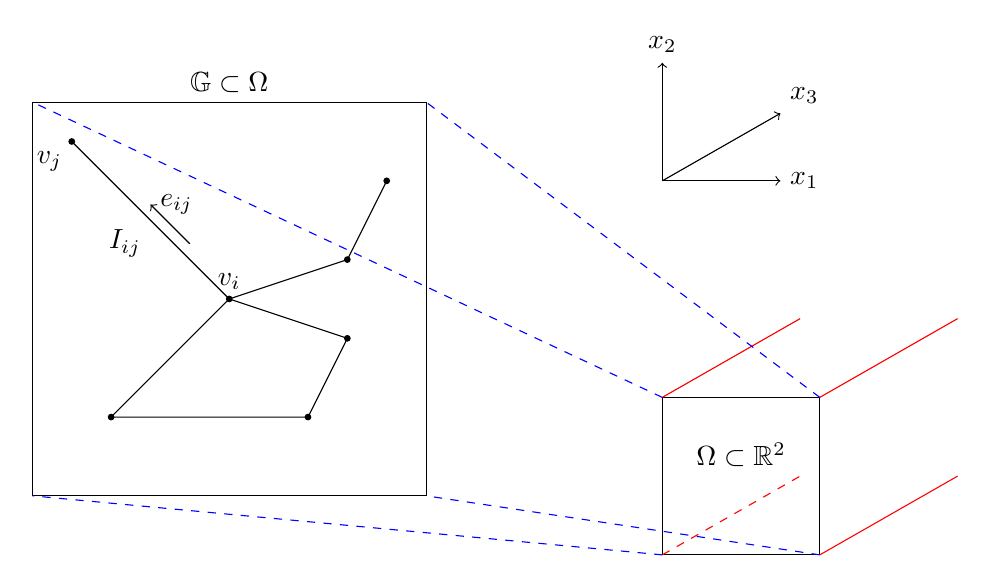
\begin{tikzpicture}
		%actual waveguide
		\begin{scope}[shift={(5,-2)}]
			\draw (0,0) rectangle (2,2);
			\node[anchor=south] at (1,1) {$\ddom\subset\reals^2$};
			%waveguide axis
			\draw[red] (2,0) -- (2+3.5/2,1);
			\draw[dashed, red] (0,0) -- (3.5/2,1);
			\draw[red] (0,2) -- (3.5/2,3);
			\draw[red] (2,2) -- (2+3.5/2,3);
		\end{scope}		
		
		%axes labels
		\begin{scope}[shift={(5,2)}, scale=0.75]
			\draw[->] (0,1) -- (2,1) node[anchor=west] {$x_1$};
			\draw[->] (0,1) -- (0,3) node[anchor=south] {$x_2$};
			\draw[->] (0,1) -- (2,1+8/7) node[anchor=south west] {$x_3$};
		\end{scope}
		
		%graph stucture
		\begin{scope}[shift={(-3,-1.25)}]
			\draw (0,0) rectangle (5,5);
			%graph edges
			\draw (2.5,2.5) -- (4,3) -- (4.5,4);
			\draw (2.5,2.5) -- (0.5,4.5);
			\draw (2.5,2.5) -- (1,1) -- (3.5,1) -- (4,2) -- cycle;
			%nodes
			\filldraw (2.5,2.5) circle (1pt) node[anchor=south] {$v_i$};	
			\filldraw (4,3) circle (1pt);	\filldraw (4.5,4) circle (1pt);
			\filldraw (0.5,4.5) circle (1pt) node[anchor=north east] {$v_j$};
			\filldraw (1,1) circle (1pt);	\filldraw (3.5,1) circle (1pt);	\filldraw (4,2) circle (1pt);
			\node[anchor=south] at (2.5,5) {$\graph\subset\ddom$};
			%labelling for I_ij
			\node[anchor=north east] at (1.5,3.5) {$I_{ij}$};
			\draw[->] (2,3.2) -- (1.5,3.7) node[anchor=west] {$e_{ij}$};
		\end{scope}
		
		%lines between waveguide pic and graph illustration
		\draw[dashed, blue] (5,-2) -- (-3,-1.25);
		\draw[dashed, blue] (7,-2) -- (2,-1.25);
		\draw[dashed, blue] (7,0) -- (2,3.75);
		\draw[dashed, blue] (5,0) -- (-3,3.75);
	\end{tikzpicture}
	\caption{\label{fig:ScalarStrucDiagram} An illustration of the wider setting for $\ddom$ with singular structure. The 2D problem will arise from considering a structure that is periodic in the $\bracs{x_1,x_2}$-plane and translation invariant in the $x_3$ direction; and taking the (Fourier and) Gelfand transforms to arrive at a family of problems posed on the 2D-period (cross-section) period cell. \tstk{move tikz code into separate file so that diagram can be reused!}}
\end{figure}

\subsection{Analysis of $\gradZero{\ddom}{\ddmes}$}
We first pursue an understanding of $\gradZero{\ddom}{\ddmes}$, as this will be crucial for helping us reduce the problem \eqref{eq:ScalarExampleStrongForm} to something more manageable.
We begin by first considering what $\gradZero{\ddom}{\ddmes}$ looks like when $\graph$ consists of only a single edge $I$ parallel to the $x_1$-axis.
In this case $\ddmes = \lambda_I$ (Lebesgue measure down $I$) and it can be deduced that 
\begin{align*}
	\gradZero{\ddom}{\lambda_I} &= 
	\clbracs{
		\begin{pmatrix} 0 \\ f	\end{pmatrix}
		\ \vert \ f\in\ltwo{\ddom}{\ddmes}
	},
\end{align*}
see for example \cite{zhikov2000extension}.
Intuitively we can think of this result as follows \tstk{use the tikzpicture you created for this!}: the smooth gradient $\grad$ (from which $\grad_\ddmes$ is constructed) details the rate of change of the function it is applied to.
The measure $\ddmes$ however can only ``see" along (or alternatively ``only cares about") what's going on along the segment $I$, as this is it's entire support.
As such $\ddmes$ can only see the change along the segment $I$, and hence we find that $\gradZero{\ddom}{\ddmes}$ consists of all the gradients that are directed perpendicular to $I$.
Furthermore any gradient orthogonal to $\gradZero{\ddom}{\ddmes}$ is directed parallel to $I$, so $\grad_\ddmes$ can only ``see" rates of change parallel to the segment $I$.
This interpretation is further reinforced by the following analysis, which characterises $\gradZero{\ddom}{\ddmes}$ when the segment $I$ is not (necessarily) parallel to the $x_1$-axis. \newline

Consider the case when $\graph$ consists of a single segment $I\subset\ddom$ with orthogonal co-ordinate system $y=\bracs{y_1,y_2}$, with $y_1$ parallel to $I$.
Let $R$ be the orthogonal change of co-ordinates $x=Ry$ with $x=\bracs{x_1,x_2}$ the orthogonal co-ordinate system along the axes. \tstk{result on rotating gradients is kind of awkwardly placed, make it fit in better.}
\begin{lemma}[Gradients under Rotation]
	Let $D\subset\reals^n$, $\phi\in C^1\bracs{D}$, and let $x=\bracs{x_j}$, $y=\bracs{y_j}$ be two co-ordinate systems for $D$, related by $x=Ry$ for a rotation $R\in\mathrm{SO}\bracs{n}$.
	Let $\grad_x$ and $\grad_y$ denote the gradient operator in the $x$ and $y$ co-ordinate systems accordingly.
	Then
	\begin{align*}
		\grad_x u &= R \grad_y u, \\
		\grad_y u &= R^{\top} \grad_x u.
	\end{align*}
\end{lemma}
\begin{proof}
	We use index notation to save explicitly writing summation symbols;
	\begin{align*}
		\bracs{\grad_x u}_j &= \pdiff{u}{x_j} = \pdiff{u}{y_k}\pdiff{y_k}{x_j} \\
		&= R_{jk}\pdiff{u}{y_k} = \bracs{\grad_y u}_j.
	\end{align*}
\end{proof}
\tstk{check notation, and cross-reference with note-book - it's not all copy and paste from before!}
If $v\in\gradZero{\ddom}{\lambda_I}$ then there exists a sequence of functions $\phi_k\in\smooth{\ddom}$ such that $\phi_k\lconv{\ltwo{\ddom}{\lambda_I}}0$ and $\grad_y\phi_k\lconv{\ltwo{\ddom}{\lambda_I}^2} v \toInfty{k}$.
Define $\psi_k = \phi_k\bracs{R^{\top}x}$, and let $\lambda_{R^{\top}I}$ denote the measure obtained from the composition $\lambda_I\circ R^{\top}$ (note that this is just the measure that supports 1D Lebesgue measure down the rotated segment).
Then using the change of variables $x=Ry$, $\psi_k\lconv{\ltwo{\ddom}{\lambda_{R^{\top}I}}}0$, and
\begin{align*}
	\grad_x\psi_k &= \grad_x\phi_k\bracs{R^{\top}x} = R^{\top}\grad_y\phi_k\bracs{y}\big\vert_{y=R^{\top}x} \\
	&\lconv{\ltwo{\ddom}{\lambda_{R^{\top}I}}} R^{\top}v\bracs{R^{\top}x} =: w\bracs{x}.
\end{align*}
Now $w$ is a gradient of zero for a segment parallel to the $x_1$ axis, and hence has the form
\begin{align*}
	w &= \begin{pmatrix} 0 \\ f \end{pmatrix}, &\quad f\in\ltwo{\ddom}{\lambda_{R^{\top}I}} \\
	\Leftrightarrow v\bracs{R^{\top}x} &= R\begin{pmatrix} 0 \\ f \end{pmatrix} &\\
	\Leftrightarrow v\bracs{y} &= R\begin{pmatrix} 0 \\ \widetilde{f} \end{pmatrix}, &\quad \widetilde{f}\in\ltwo{\ddom}{\lambda_I}.
\end{align*}
This confirms that 
\begin{align*}
	\gradZero{\ddom}{\lambda_I} &= \clbracs{R\begin{pmatrix} 0 \\ \widetilde{f} \end{pmatrix} \ \vert \ \widetilde{f}\in\ltwo{\ddom}{\lambda_I}} \\
	&= \clbracs{g\in\ltwo{\ddom}{\lambda_I}^2 \ \vert \ g\cdot e_{I} = 0}
\end{align*}
where $e_I$ is the unit vector directed along the segment $I$.

%\subsubsection{Graphs with Multiple Edges}
%Of course the results so far only describe the set of gradients of zero for graphs with single edges, however we can use this understanding of single edges to build up an understanding of what happens to gradients of zero when we have a more interesting graph.
%In particular, we want to show that for a (multiple-edge) graph $\graph$ and $\ddmes$ supporting it's edges, we have that
%\begin{align*}
%	\gradZero{\ddom}{\ddmes} &= \clbracs{g\in\ltwo{\ddom}{\ddmes} \ \vert \ g\vert_{I_{ij}}\cdot e_{ij}=0 \ \forall I_{ij}\in E}.
%\end{align*}
%This provides an edge-wise characterisation of the set of gradients of zero; any gradient of zero for the whole graph has (upon restriction) the same form as a gradient of zero along each edge of the graph.
%Here $g\vert_{I_{ij}}$ denotes the restriction of the function $g$ to the edge $I_{ij}$, and $e_{ij}$ denotes the unit vector (directed $v_i$ to $v_j$) along $I_{ij}$.
%For convenience, we denote the set on the right hand side of the equality by $B$.
%The inclusion $\gradZero{\ddom}{\ddmes} \subset B$ follows quickly:
%\begin{prop} \label{prop:Grad0IncB}
%	For $B=\clbracs{g\in\ltwo{\ddom}{\ddmes} \ \vert \ g\vert_{I_{ij}}\cdot e_{ij}=0 \ \forall I_{ij}\in E}$, we have
%	\begin{align*}
%		\gradZero{\ddom}{\ddmes}\subset B
%	\end{align*}
%\end{prop}
%\begin{proof}
%	If $g\in\gradZero{\ddom}{\ddmes}$ then there exists a sequence of smooth functions $\phi_k$ such that $\phi_k\lconv{\ltwo{\ddom}{\ddmes}}0, \grad\phi_k\lconv{\ltwo{\ddom}{\ddmes}^2}g$.
%	Thus, due to the structure of $\ddmes$
%	\begin{align*}
%		\sum_{I_{ij}}\integral{I_{ij}}{\abs{\phi_k}^2}{\lambda_{I_{ij}}} &= \integral{\ddom}{\abs{\phi_k}^2}{\ddmes} \\
%		&\rightarrow 0 \toInfty{k}
%	\end{align*}
%	and as every term in the sum is non-negative, each term must also be tending to 0.
%	Thus 
%	\begin{align*}
%		\phi_k\lconv{\ltwo{\ddom}{\lambda_{I_{ij}}}}0 \ \forall I_{ij}\in E.
%	\end{align*}
%	Similarly
%	\begin{align*}
%		\sum_{I_{ij}}\integral{I_{ij}}{\abs{\grad\phi_k - g\vert_{I_{ij}}}^2}{\lambda_{I_{ij}}} &= \integral{\ddom}{\abs{\grad\phi_k - g}^2}{\ddmes} \\
%		&\rightarrow 0 \toInfty{k}
%	\end{align*}	
%	and hence 
%	\begin{align*}
%		\grad\phi_k\lconv{\ltwo{\ddom}{\lambda_{I_{ij}}}^2} g\vert_{I_{ij}} \ \forall I_{ij}\in E.
%	\end{align*}
%	Hence $g\in B$.
%\end{proof}
%
%The reverse inclusion requires some further preliminary results before it can be proven.
%\begin{lemma}[Extension of Gradients on Segments to Whole Graph] \label{lem:SegGradExtend}
%	Let $I_{ij}^{n} = \clbracs{x\in I_{ij} \ \vert \ \mathrm{dist}\bracs{x, \partial I_{ij}}\geq\recip{n}}$.
%	Suppose further that we have a function $g\in\ltwo{\ddom}{\ddmes}$ with $g=0$ on $\graph\setminus I_{ij}^{n}$ and $g\cdot e_{ij}=0$ on $I_{ij}^{n}$.
%	Then $g\in\gradZero{\ddom}{\ddmes}$.
%\end{lemma}
%\begin{proof}
%	As $g\cdot e_{ij}=0$ on $I_{ij}^{n}$ and $g=0$ on $I_{ij}\setminus I_{ij}^{n}$, we have that $g\cdot e_{ij}=0$ on $I_{ij}$ and hence $g\in\gradZero{\ddom}{\lambda_{I_{ij}}}$.
%	So we can find a sequence of smooth functions $\phi_k$ with the properties $\phi_k\lconv{\ltwo{\ddom}{\lambda_{I_{ij}}}}0$, $\grad\phi_k\lconv{\ltwo{\ddom}{\lambda_{I_{ij}}}^2}g\vert_{I_{ij}}$.
%	Now let $\chi_{ij}^{n}\in\smooth{\ddom}$ be the function such that
%	\begin{align*}
%		\chi_{ij}^{n}\bracs{x} &\in [0,1], \\
%		\chi_{ij}^{n} = 1 &\text{ whenever } \mathrm{dist}\bracs{x, I_{ij}^n}\leq \recip{3n} \\
%		\chi_{ij}^{n} = 0 &\text{ whenever } \mathrm{dist}\bracs{x, I_{ij}^n}\geq \frac{2}{3n}
%	\end{align*}
%	\begin{figure}
%		\centering
%		\begin{tikzpicture}
%			\begin{scope}[scale=2, rotate=-26.565]
%				\draw (0,0) -- (6,3);
%				\filldraw (0,0) circle (1pt) node[anchor=north] {$v_i$};
%				\filldraw (6,3) circle (1pt) node[anchor=south] {$v_j$};
%				\draw[red, line width=2pt] (1,0.5) -- (5,2.5);
%				\draw[dashed] (1-1/5,0.5+2/5) -- (5-1/5,2.5+2/5) to[out=26.565, in=26.565] (5+1/5,2.5-2/5) -- (1+1/5,0.5-2/5) to[out=180+26.565, in=180+26.565] cycle;
%				\draw[dashed] (1-2/5,0.5+4/5) -- (5-2/5,2.5+4/5) to[out=26.565, in=26.565] (5+2/5,2.5-4/5) -- (1+2/5,0.5-4/5) to[out=180+26.565, in=180+26.565] cycle;
%			\end{scope}
%			\node at (6,0.25) {$\chi_{ij}^{n}=1$};
%			\node at (6,1.25) {$0\leq\chi_{ij}^{n}\leq1$};
%			\node at (6,2.25) {$\chi_{ij}^{n}=0$};
%			\draw[->] (3,0) -- (3,-4/5);
%			\draw[->] (3,-4/5) -- (3,0);
%			\node[anchor=west] at (3,-2/5) {$\recip{3n}$};
%			\node[anchor=west] at (10,-6/5) {$\frac{2}{3n}$};
%			\draw[->] (10,0) -- (10,-9/5);
%			\draw[->] (10,-9/5) -- (10,0);
%			\draw[->] (13.416,-0.5) -- (11.18,-0.5);
%			\draw[->] (11.18,-0.5) -- (13.416,-0.5);
%			\node[anchor=north] at (12.5,-0.5) {$\recip{n}$};
%		\end{tikzpicture}
%		\caption{\label{fig:chiDiagram} The function $\chi_{ij}^n$ on the region surrounding the segment $I_{ij}^n$. Should another edge of $\graph$ lie in the region $\clbracs{x \ \vert \ \mathrm{dist}\bracs{x,I_{ij}^{n}}\leq\frac{2}{3n}}$, we can simply apply a rescaling to the argument of $\chi_{ij}^n$ to avoid this issue.}
%	\end{figure}
%	Note that since $\graph$ is finite, we can assume without loss of generality that the only edge of $\graph$ that lies in the support of $\chi_{ij}^n$ is $I_{ij}$, otherwise we apply a scaling to the argument of $\chi_{ij}^n$ to avoid this issue.
%	Furthermore, $\abs{\grad\chi_{ij}^{n}}$ is bounded by a constant that depends on $n$ only.
%	Now consider the sequence $\psi_k = \chi_{ij}^{n}\phi_k$.
%	We have that
%	\begin{align*}
%		\integral{\ddom}{\abs{\psi_k}^2}{\ddmes} = \integral{I_{ij}}{\abs{\chi_{ij}^{n}\phi_k}^2}{\lambda_{I_{ij}}}
%		\leq \integral{I_{ij}}{\abs{\phi_k}^2}{\lambda_{I_{ij}}} \rightarrow0 \toInfty{k},
%	\end{align*}
%	which is one of the desired convergence results for $\psi_k$.
%	For the other convergence result we need, observe that
%	\begin{align*}
%		\integral{\ddom}{\abs{\phi_k\grad\chi_{ij}^{n}}^2}{\ddmes} &= \integral{I_{ij}}{\abs{\phi_k\grad\chi_{ij}^{n}}^2}{\lambda_{I_{ij}}} \\
%		&\leq \sup_{I_{ij}}\bracs{\abs{\grad\chi_{ij}^{n}}^{2}}\integral{I_{ij}}{\abs{\phi_{k}}^{2}}{\ddmes} \\
%		&\rightarrow 0 \toInfty{k}
%	\end{align*}
%	because $\abs{\grad\chi_{ij}^{n}}$ depends on $n$ only.
%	Additionally
%	\begin{align*}
%		\integral{\ddom}{\abs{\chi_{ij}^n\grad\phi_k - g\vert_{I_{ij}}}^2}{\ddmes} &= \integral{I_{ij}}{\abs{\chi_{ij}^n\grad\phi_k - g\vert_{I_{ij}}}^2}{\lambda_{I_{ij}}} \\
%		&= \integral{I_{ij}\setminus I_{ij}^n}{\abs{\chi_{ij}^n\grad\phi_k - g\vert_{I_{ij}}}^2}{\lambda_{I_{ij}}} + \integral{I_{ij}^n}{\abs{\chi_{ij}^n\grad\phi_k - g\vert_{I_{ij}}}^2}{\lambda_{I_{ij}}} \\
%		&= \integral{I_{ij}\setminus I_{ij}^n}{\abs{\chi_{ij}^n\grad\phi_k}^2}{\lambda_{I_{ij}}} +  \integral{I_{ij}^n}{\abs{\grad\phi_k - g\vert_{I_{ij}}}^2}{\lambda_{I_{ij}}} \\
%		&\leq \integral{I_{ij}\setminus I_{ij}^n}{\abs{\grad\phi_k}^2}{\lambda_{I_{ij}}} +  \integral{I_{ij}^n}{\abs{\grad\phi_k - g\vert_{I_{ij}}}^2}{\lambda_{I_{ij}}} \\
%		&= \integral{I_{ij}\setminus I_{ij}^n}{\abs{\grad\phi_k - g\vert_{I_{ij}}}^2}{\lambda_{I_{ij}}} +  \integral{I_{ij}^n}{\abs{\grad\phi_k - g\vert_{I_{ij}}}^2}{\lambda_{I_{ij}}} \\
%		&= \integral{I_{ij}}{\abs{\grad\phi_k - g\vert_{I_{ij}}}^2}{\lambda_{I_{ij}}} \rightarrow0 \toInfty{k},
%	\end{align*}
%	where we have made use of the fact that $g\vert_{I_{ij}}=0$ on $I_{ij}\setminus I_{ij}^n$ and the various properties of $\chi_{ij}^n$.
%	Armed with these inequalities, we have that
%	\begin{align*}
%		\integral{\ddom}{\abs{\grad\psi_k - g\vert_{I_{ij}}}^2}{\ddmes} &= \integral{\ddom}{\abs{\chi_{ij}^n\grad\phi_k + \phi_k\grad\chi_{ij}^n - g\vert_{I_{ij}}}^2}{\ddmes} \\
%		&\leq 2\integral{\ddom}{\abs{\phi_k\grad\chi_{ij}^n}^2}{\ddmes} + 2\integral{\ddom}{\abs{\chi_{ij}^n\grad\phi_k - g\vert_{I_{ij}}}^2}{\ddmes} \\
%		&\rightarrow0 \toInfty{k}.
%	\end{align*}
%	Thus, $\psi_k$ is a sequence of smooth functions such that
%	\begin{align*}
%		\psi_k \lconv{\ltwo{\ddom}{\ddmes}} 0, &\quad
%		\grad\psi_k \lconv{\ltwo{\ddom}{\ddmes}^2} g
%	\end{align*}
%	and hence, $g\in\gradZero{\ddom}{\ddmes}$.
%\end{proof}
%
%The other result we need is a convergence result for a particular form of function we will utilise in the proof.
%Let the function $\eta\in\smooth{\ddom}$ with the properties
%\begin{align*}
%	\eta\bracs{x} &\in [0,1], \\
%	\eta = 0 &\text{ whenever } \abs{x}\leq 1, \\
%	\eta = 1 &\text{ whenever } \abs{x}\geq 2.
%\end{align*}
%Then for each $v_i\in V$ and $n\in\naturals$, we define
%\begin{align*}
%	\eta_i\bracs{x} = \eta\bracs{x-v_i}, &\quad \eta_i^n\bracs{x} = \eta_i\bracs{nx}
%\end{align*}
%which are clearly both smooth functions by composition.
%\begin{lemma}[Convergence of $\eta_i^n$ in $\ltwo{\ddom}{\ddmes}$] \label{lem:etaConv}
%	For any $v_i\in V$, $\eta_i^n \rightarrow 1$ in $\ltwo{\ddom}{\ddmes} \toInfty{n}$.
%\end{lemma}
%\begin{proof}
%	We can directly prove this convergence by estimating the integral from above:
%	\begin{align*}
%		\begin{split}
%			\integral{\ddom}{\abs{\eta_i^n-1}^2}{\ddmes} &= \integral{\graph\setminus B_{2/n}\bracs{v_{i}}}{\abs{\eta_{i}^{n}-1}^{2}}{\ddmes} + \integral{\graph \cap \bracs{B_{2/n}\bracs{v_{i}} \setminus B_{1/n}\bracs{v_{i}}}}{\abs{\eta_{i}^{n}-1}^{2}}{\ddmes} \\ + &\integral{\graph\cap B_{1/n}\bracs{v_{i}}}{\abs{\eta_{i}^{n}-1}^{2}}{\ddmes} \\
%			&= \integral{\graph\setminus B_{2/n}\bracs{v_{i}}}{0}{\ddmes} + \integral{\graph \cap \bracs{B_{2/n}\bracs{v_{i}} \setminus B_{1/n}\bracs{v_{i}}}}{\abs{\eta_{i}^{n}-1}^{2}}{\ddmes} \\ + &\integral{\graph\cap B_{1/n}\bracs{v_{i}}}{}{\ddmes} \\
%			&\leq \integral{\graph \cap \bracs{B_{2/n}\bracs{v_{i}} \setminus B_{1/n}\bracs{v_{i}}}}{}{\ddmes} + \integral{\graph\cap B_{1/n}\bracs{v_{i}}}{}{\ddmes} \\
%			&=\integral{\graph\cap B_{2/n}\bracs{v_{i}}}{}{\ddmes} = \ddmes\bracs{\graph\cap B_{2/n}\bracs{v_{i}}} \\
%			&\leq \frac{4 \abs{E}}{n} \rightarrow0 \toInfty{n}.
%		\end{split}
%	\end{align*}
%	The last line following because each edge of $\graph$ can intersect $B_{2/n}\bracs{v_i}$ on a segment of length $\leq\frac{4}{n}$.
%\end{proof}
%
%We are now ready to prove that $B\subset\gradZero{\ddom}{\ddmes}$.
%\begin{prop} \label{prop:BIncGrad0}
%	For $B=\clbracs{g\in\ltwo{\ddom}{\ddmes} \ \vert \ g\vert_{I_{ij}}\cdot e_{ij}=0 \ \forall I_{ij}\in E}$, we have
%	\begin{align*}
%		B \subset \gradZero{\ddom}{\ddmes}
%	\end{align*}
%\end{prop}
%\begin{proof}
%	Take $g\in B$, and define a family of functions $g_{n}$ by
%	\begin{align*}
%		g_{n}\bracs{x} &= \recip{2}\sum_{i\in V}\sum_{i\sim j}\eta_{i}^{n}\bracs{x}\eta_{j}^{n}\bracs{x}g\vert_{I_{ij}}\bracs{x}
%	\end{align*}
%	where the notation $i\sim j$ means that there is an edge $(i,j)\in E$, and the sum is taken over such edges.
%	Recall that $\graph$ was assumed finite, so there are no convergence issues with the double sum.
%	Then for each $i,j$ with $i\sim j$, the function $\eta_{i}^{n}\eta_{j}^{n}g\vert_{I_{ij}}$ satisfies the hypothesis of \ref{lem:SegGradExtend}, so $\eta_{i}^{n}\eta_{j}^{n}g\vert_{I_{ij}}\in\gradZero{\ddom}{\ddmes}$.
%	Furthermore, as $\gradZero{\ddom}{\ddmes}$ is a linear subspace of $\ltwo{\ddom}{\ddmes}^{2}$, $g_{n}\in\gradZero{\ddom}{\ddmes}$ too, for all $n$.
%	By closure of $\gradZero{\ddom}{\ddmes}$; $g_{n}$ converges in $\gradZero{\ddom}{\ddmes}$ provided it converges at all, so it remains to show that $g_{n}\lconv{\ltwo{\ddom}{\ddmes}^2} g \toInfty{n}$.
%	However with the result of \ref{lem:etaConv}, we have that $\eta_{i}^{n}\eta_{j}^{n}g\vert_{I_{ij}}\lconv{\ltwo{\ddom}{\ddmes}^2} g\vert_{I_{ij}}$ and hence
%	\begin{align*}
%		g_{n} \lconv{\ltwo{\ddom}{\ddmes}^2} &\recip{2}\sum_{i\in V}\sum_{j\sim i}g\vert_{I_{ij}} = g \toInfty{n},
%	\end{align*}
%	so $g\in\gradZero{\ddom}{\ddmes}$.
%\end{proof}
%
%\subsection{Reduction to a system of scalar equations} \label{sec:ScalarReduceEdgeEqns}
%We now turn our attention back to \eqref{eq:ScalarExampleStrongForm}.
%Recall that we interpret this in the weak sense, namely a pair $\bracs{u,\grad_\ddmes u}$ solves \eqref{eq:ScalarExampleStrongForm} if and only if
%\begin{align} \label{eq:ScalarExampleWeakForm}
%	\integral{\ddom}{\grad_\ddmes u \cdot \grad\phi}{\ddmes} &= \omega^2\integral{\ddom}{u\phi}{\ddmes} \quad \forall\phi\in\smooth{\ddom}.
%\end{align}
%\tstk{again reiterate Gelfand/Fourier and the case we are considering. Also how can we guarantee solutions to this system?}
%We want to find an alternative but equivalent system to \eqref{eq:ScalarExampleWeakForm} that we can use in numerical schemes (as the measure $\ddmes$ prevents implementations via finite elements, for example) or is more tractable to an analytic approach.
%To this end we look to work from \eqref{eq:ScalarExampleWeakForm} and employ our previous analysis to find an alternative problem. \newline
%
%We begin by re-writing \eqref{eq:ScalarExampleWeakForm} by appealing to the nature of $\ddmes$;
%\begin{align} \label{eq:ScalarExampleSumOfInts}
%	0 &= \recip{2}\sum_{I_{ij}\in E}\integral{\ddom}{\grad_\ddmes u \cdot \grad\phi - \omega^2 u\phi}{\lambda_{ij}}.
%\end{align}
%Note that $I_{ij},I_{ji}\in E$ are the same edge of the graph $\graph$, which is what gives us the factor of a half.
%Of course we may simply drop this factor of a half, and understand the sum as being over unique edges, which we henceforth do.
%Next recall the notation introduced for the edge $I_{ij}$; we denote by $e_{ij}$ the unit vector along $I_{ij}$ pointing from $v_i$ to $v_j$,
%\begin{align*}
%	e_{ij} = \frac{v_j-v_i}{\norm{v_j-v_i}_2}.
%\end{align*}
%We define the map 
%\begin{align*}
%	r_{ij}:\sqbracs{0,\abs{I_{ij}}} &\rightarrow I_{ij}, \\
%	r_{ij}\bracs{t} &= v_i + te_{ij}
%\end{align*}
%so $r'\bracs{t}=e_{ij}$.
%Note that $r$ is therefore an admissible change of variables from $\sqbracs{0,\abs{I_{ij}}}$ to $I_{ij}$.
%To prevent cluttered notation, we use an overhead tilde to denote composition with $r_{ij}$, so for example $\tilde{\phi}=\phi\circ r_{ij}$.
%We next look at how to deal with each integral term.
%Without loss of generality we can assume that each $I_{ij}$ is parallel to the $x_1$-axis by performing a rotation, and we denote by $u_{ij}\in\ltwo{\ddom}{\lambda_{ij}}$ the function such that $u_{ij}=u$ on the (potentially rotated) edge $I_{ij}$.
%$u_{ij}$ can be thought of as the $ij$\textsuperscript{th}-part of $u$, or the part of $u$ down the edge $I_{ij}$ - this separation of $u$ onto separate functions on the edges of $\graph$ will prove useful in what follows.
%Although we do not need to make this simplification since we have information about $\gradZero{\ddom}{\lambda_{ij}}$, it is helpful to do so in the following analysis.
%In fact the information about $\gradZero{\ddom}{\lambda_{ij}}$ is necessary to perform the rotation we would use, and retain equivalence of the resulting problem to the original. \newline
%
%With this simplification, we examine the term
%\begin{align*}
%	\integral{\ddom}{\grad_\ddmes u_{ij}\cdot\grad\phi}{\lambda_{ij}}.
%\end{align*}
%We know that the solution to \eqref{eq:ScalarExampleWeakForm} satisfies $\grad_\ddmes u \perp \gradZero{\ddom}{\ddmes}$ and so $\grad_\ddmes u_{ij} \perp \gradZero{\ddom}{\lambda_{ij}}$ by our analysis of gradients of zero.
%Thus let us suppose that $\grad_\ddmes u_{ij} = \bracs{\alpha, \beta}^{\top}$.
%Recalling the characterisation of $\gradZero{\ddom}{\lambda_{ij}}$ when $I_{ij}$ is parallel to the $x_1$-axis, we require that
%\begin{align*}
%	0 &= \integral{\ddom}{\grad_\ddmes u_{ij} \cdot \begin{pmatrix} 0 \\ f \end{pmatrix}}{\lambda_{ij}} \quad \forall f\in\ltwo{\ddom}{\lambda_{ij}}, \\
%	\Rightarrow 0 &= \integral{I_{ij}}{\beta f}{\lambda_{ij}}
%	= \int_{0}^{\abs{I_{ij}}}\widetilde{\beta}\widetilde{f}\md t.
%\end{align*}
%As $\widetilde{f}$ is arbitrary, we conclude that $\widetilde{\beta}=0$ and hence $\beta=0$.
%Thus $\grad_\ddmes u_{ij} = \bracs{\alpha, 0}^{\top}$; we now show that $\alpha$ is related to the distributional derivative of the function $\widetilde{u}_{ij}$.
%Notice that for any smooth function $\phi$ we have that
%\begin{align*} \labelthis\label{eq:PartialToTDiff}
%	\partial_t\widetilde{\phi}(t) &= \grad\phi\bracs{r_{ij}(t)}\cdot r'_{ij}(t) = \partial_1\phi\bracs{r_{ij}(t)} \\
%	&= \widetilde{\partial_1\phi}(t),
%\end{align*}
%as $r'_{ij}=e_{ij}=\bracs{1,0}^{\top}$.
%Now as $u_{ij}\in\ltwo{\ddom}{\lambda_{ij}}$ we can find smooth functions $\alpha_n$ such that
%\begin{align*}
%	\alpha_n\lconv{\ltwo{\ddom}{\lambda_{ij}}}u_{ij}, \quad \grad\alpha_n\lconv{\ltwo{\ddom}{\lambda_{ij}}^2}\begin{pmatrix} \alpha \\ 0	\end{pmatrix}.
%\end{align*}
%Exploiting the change of variables $r_{ij}$ and writing these statements using integrals converging in $\reals$ implies
%\begin{align*}
%	\int_0^{\abs{I_{ij}}}\abs{\widetilde{\alpha}-\widetilde{u}_{ij}}^2 \md t &\rightarrow 0, \\
%	\int_0^{\abs{I_{ij}}}\abs{\partial_t\widetilde{\alpha}_n - \widetilde{\alpha}}^2 \md t = \int_0^{\abs{I_{ij}}}\abs{\partial_1\widetilde{\alpha}_n - \widetilde{\alpha}}^2 \md t &\rightarrow 0, \\
%	\int_0^{\abs{I_{ij}}}\abs{\partial_2\widetilde{\alpha}_n}^2 \md t &\rightarrow 0, \toInfty{n}.
%\end{align*}
%In particular the first two convergences imply that $\widetilde{\alpha}=\widetilde{u}'_{ij}$; that is that $\widetilde{\alpha}$ is the distributional derivative of $\widetilde{u}_{ij}\in\gradSob{\sqbracs{0,\abs{I_{ij}}}}{t}$.
%Using the notation $u'_{ij}$ for the $\ltwo{\ddom}{\lambda_{ij}}$ function such that $u'_{ij} = \widetilde{u}'_{ij}\circ r_{ij}^{-1}$, we can write $\grad_\ddmes u_{ij} = \bracs{u'_{ij}, 0}^{\top}$.
%In light of this we see that
%\begin{align*}
%	\integral{\ddom}{\grad_\ddmes u_{ij} \cdot \grad\phi - \omega^2 u_{ij}\phi}{\lambda_{ij}}
%	&= \int_0^{\abs{I_{ij}}}\widetilde{u}'_{ij}\widetilde{\phi}' - \omega^2\widetilde{u}_{ij}\widetilde{\phi} \md t.
%\end{align*}
%
%Equipped with this knowledge, we are able to transform \eqref{eq:ScalarExampleSumOfInts} into
%\begin{align} \label{eq:ScalarExampleLebesgueIntegrals}
%	0 &= \sum_{I_{ij}\in E}\int_0^{\abs{I_{ij}}}\widetilde{u}'_{ij}\widetilde{\phi}' - \omega^2\widetilde{u}_{ij}\widetilde{\phi} \md t.
%\end{align}
%The choice of $\phi$ was arbitrary so in particular \eqref{eq:ScalarExampleLebesgueIntegrals} must hold when $\mathrm{supp}\bracs{\phi}$ contains precisely one edge $I_{ij}$, meaning that we have
%\begin{align*}
%	0 &= \int_0^{\abs{I_{ij}}}\widetilde{u}'_{ij}\widetilde{\phi}' - \omega^2\widetilde{u}_{ij}\widetilde{\phi} \md t, \quad \forall I_{ij}\in E, \ \forall \phi\in\smooth{\ddom}.
%\end{align*}
%That is to say, we have arrived at a system of differential equations (``edge equations") for $\widetilde{u}_{ij}$ (the ``edge solutions").
%This weak formulation admits numerical solution by (for example) finite elements, providing us with a method to recover the original function $u$.
%If we assume more regularly of $u$, for example assume that $u\in C^2\bracs{\ddom}$ so the second derivative of $u$ exists in the strong sense we can obtain a system of ODEs in the edge solutions $\widetilde{u}_{ij}$, complete with boundary conditions.
%We obtain one (second-order) differential equation for each edge $I_{ij}$ by integrating each edge equation by parts;
%\begin{align*}
%	0 &= \int_0^{\abs{I_{ij}}}\widetilde{u}'_{ij}\widetilde{\phi}' - \omega^2\widetilde{u}_{ij}\widetilde{\phi} \md t, \quad \forall\phi\in\smooth{\ddom} \\
%	&= \int_0^{\abs{I_{ij}}} \bracs{\widetilde{u}''_{ij} + \omega^2\widetilde{u}_{ij}}\widetilde{\phi} \md t. \\
%	\Rightarrow 0 &= \widetilde{u}''_{ij} + \omega^2\widetilde{u}_{ij}.
%\end{align*}
%As we have assumed at least $C^2$ regularity of $u$ we require that $u$ be continuous at the vertices $v_i$ and so we must have that
%\begin{align*}
%	\widetilde{u}_{ij}\vert_{v_i} &= \widetilde{u}_{ik}\vert_{v_i} \quad \text{whenever } i\sim j \text{ and } i\sim k,
%\end{align*}
%which is simply a matching condition of the solution at the vertices.
%The vertical bar notation is used to denote evaluation, so $\widetilde{u}_{ij}\vert_{v_i}$ denotes evaluation of $\widetilde{u}_{ij}\bracs{t}$ at whichever $t$ such that $r_{ij}\bracs{t} = v_i$. 
%The other boundary conditions can be found by considering $\phi$ such that $\mathrm{supp}\bracs{\phi}$ contains precisely one of the vertices $v_k$, and then integrating \eqref{eq:ScalarExampleLebesgueIntegrals} by parts and considering the boundary term:
%\begin{align*}
%	0 &= \sum_{I_{ij}\in E}\int_0^{\abs{I_{ij}}}\widetilde{u}'_{ij}\widetilde{\phi}' - \omega^2\widetilde{u}_{ij}\widetilde{\phi} \md t \\
%	&= \sum_{I_{ij}\in E}\int_0^{\abs{I_{ij}}} \bracs{\widetilde{u}''_{ij} + \omega^2\widetilde{u}_{ij}}\widetilde{\phi} \md t + \sum_{I_{ij}\in E}\sum_{i\sim j}\sqbracs{\widetilde{u}'_{ij}\widetilde{\phi}}\big\vert_{v_i} \\
%	&= \sum_{I_{ij}\in E}\sum_{i\sim j}\sqbracs{\widetilde{u}'_{ij}\widetilde{\phi}}\big\vert_{v_i} \\
%	&= \sum_{k\sim j}\widetilde{u}'_{kj}\vert_{v_k}\widetilde{\phi}\vert_{v_k}, \\
%	\Rightarrow 0 &= \sum_{k\sim j}\widetilde{u}'_{kj}\vert_{v_k}.
%\end{align*}
%That is we obtain a Kirchoff condition on the derivatives of the edge solutions at each of the vertices.
%These conditions provide us with a complete system of differential equations and boundary conditions; observe that for each edge equation we can select one of it's vertices and associate one matching condition and one Kirchoff condition at that vertex.
%
%\section{Chapter Summary}
%The work in this section largely builds off that of \tstk{references!!}, before pursuing an example that will be relevant in the later sections.
%We have introduced the theory behind the kinds of mathematical problems and their associated spaces.
%One constructs the Sobolev spaces $\gradSob{D}{\nu}$ using closure of the set of $\smooth{D}$ functions and their gradients, the cost of which is uniqueness of the $\nu$-gradients, $\grad_\nu$.
%However one can characterise all the gradients of a given function $u\in\gradSob{D}{\nu}$ by finding the unique $\grad_\nu u$ which is perpendicular to the set of $\nu$-gradients of 0, $\gradZero{D}{\nu}$.
%As such understanding the structure of $\gradZero{D}{\nu}$ is central to finding solutions to problems posed in $\gradSob{D}{\nu}$. \newline
%
%The example provided in section \ref{sec:ScalarExample} demonstrates how this theory can be employed to reduce an abstract problem involving $\nu$-gradients to an equivalent problem which involves more familiar (or ``classical") objects.
%Starting from the problem \eqref{eq:ScalarExampleStrongForm}, one can obtain the system \eqref{eq:ScalarExampleLebesgueIntegrals} which can be approached numerically via schemes like finite elements, and the solution to the original problem can be recovered.
%Under further regularly assumptions, one can even obtain systems of ODEs which may prove admissible to an analytic approach and even yield exact solutions. \newline
%
%We will be looking to extend the concepts introduced here when we move towards considering systems of vector-valued functions, which are widely used in the description of physical systems.
%Many of the argumentative techniques that we have employed in this section will provide inspiration for the arguments we employ in chapter \ref{ch:3VectorEqns}.

%
%\chapter{Vector Equations} \label{ch:VectorEqns}
Chapter \ref{ch:ScalarEqns} introduced the theory of Sobolev spaces $\gradSob{D}{\nu}$ with respect to arbitrary (Borel) measures $\nu$, and how we can make sense of the notion of ``derivative" and pose problems in these spaces.
Also investigated was how (under suitable regularity assumptions) the variational problems that can be posed are reduced to Quantum Graph problems, when the measure $\nu$ supports a graph embedded into the domain $D$. \newline

In this chapter we look to develop this theory to handling vector-valued systems of equations, which necessitates developing theory for the associated curl- and divergence-operations, as well as the associated Sobolev spaces.
We begin with the definition and construction of these spaces, during which we will demonstrate parallels with the previously seen concepts of ``tangential-gradients".
In fact, many of the arguments in this chapter will be inspired or grounded in the approaches taken in chapter \ref{ch:ScalarEqns}.
After this we will discuss slightly altered versions of these spaces, which will arise from considering the wave-propagation problems of interest to us.
We will provide a worked example in this context, and once again demonstrate how we can obtain a Quantum Graphs problem from a variational formulation when the measure $\nu$ supports a graph in the $\bracs{x_1,x_2}$-plane.

\section{Vector Sobolev Spaces} \label{sec:VectorSobSpaces}
In this section we discuss the construction of Sobolev spaces of vector-valued functions that possess curls (in some sense) with respect to an arbitrary (Borel) measure $\nu$.
In later sections we will adapt the construction of these spaces to suit our physical wave-guide and photonic-fibre systems; by taking a Fourier transform along the axis of the wave-guide and also incorporating the quasi-momentum that arises from taking a Gelfand transform in the cross-section.
The reader is invited to bear in mind the arguments employed in section \ref{sec:ScalarSobSpaces} throughout this section. \newline

Let $D\subset\reals^3$ be our 3D-domain, and let $\nu$ be an arbitrary (Borel) measure on $D$.
Let $W=W\bracs{D,\md\nu}$ be the closure of the set of pairs $\bracs{\phi, \curl{}\phi}$ in $\ltwo{D}{\nu}^3\times\ltwo{D}{\nu}^3$ for $\phi\in\smooth{D}$.
Given that this is essentially the same construction as in section \ref{sec:ScalarSobSpaces}, it is unsurprising to learn that some work must be done before the element $c$ in the pair $\bracs{u,c}\in W$ can be thought of as a ``curl".
Indeed we actually have the same problem as in the gradient case; if both $\bracs{u,c_1}, \bracs{0, c_2}\in W$ then $\bracs{u,c_1+c_2}\in W$, and so we define the set of $\nu$-curls of zero as
\begin{align*}
	\curlZero{D}{\nu} &:= \clbracs{ c\in\ltwo{D}{\nu}^3 \ \vert \ \bracs{0,c}\in W }, \\
	&= \clbracs{ c\in\ltwo{D}{\nu}^3 \ \vert \ \exists\phi\in\bracs{\smooth{D}}^3 \text{ s.t. } \phi_n\lconv{\ltwo{D}{\nu}^3}0, \curl{}\phi_n\lconv{\ltwo{D}{\nu}^3}c }
\end{align*}
Fortunately we have the same methodology available to us as in the gradient case, to allow us address this issue.
That is, we observe that $\curlZero{D}{\nu}$ is a closed linear subspace of $\ltwo{D}{\nu}^3$ so we can decompose
\begin{align*}
	\ltwo{D}{\nu}^3 = \curlZero{D}{\nu}^\perp \oplus \curlZero{D}{\nu}.
\end{align*}
Hence every $u\in\ltwo{D}{\nu}^3$ has a unique tangential $\nu$-curl, $\curl{\nu} u$ such that every $\bracs{u,c}\in W$ can be written in the form $\bracs{u, \curl{\nu}u + \widetilde{c}}\in W$ for some $\widetilde{c}\in\curlZero{D}{\nu}$.
Thus we can define the Sobolev space of functions $u$ with $\nu$-curls by
\begin{align*}
	\curlSob{D}{\nu} := \clbracs{ \bracs{u,\curl{\nu}u}\in W },
\end{align*}
and although elements of this space are technically pairs, it is sufficient to specify only the first component $u$ to identify the pair.
We can also pose problems in this space using a variational formulation as was done in section \ref{sec:ScalarSobSpaces}, we write
\begin{align*}
	\curl{\nu}\bracs{A\curl{\nu}u} + u &= f, \quad u\in\curlSob{D}{\nu},
\end{align*}
and interpret this as the variational problem of finding $u\in\curlSob{D}{\nu}$ such that
\begin{align*}
	\integral{D}{ A\bracs{\curl{\nu}u}\cdot\overline{\bracs{\curl{}\phi}} + u\overline{\phi}}{\nu} &= \integral{D}{ f\overline{\phi} }{\nu}, \quad \forall\phi\in\bracs{\smooth{D}}^3.
\end{align*}
Such problems actually serve as the motivation for the notion of the tangential curl that is provided in the same way as tangential gradients were motivated.
The elliptic matrix $A$ simply requires us to write $A\curl{\nu}u$ for the element in $\curlZero{D}{\nu}^\perp$, the details again being analogous to those in section \ref{sec:ScalarSobSpaces} for gradients. \newline

The problem that we shall be focusing on throughout this chapter is the colloquially-named ``curl of the curl" equation 
\begin{align} \label{eq:curlOfCurlEqn}
	\curl{\nu}\bracs{A\curl{\nu}u} = f, &\quad u\in\curlSob{D}{\nu}, f\in\ltwo{D}{\nu}^3,
\end{align}
typically arising from the study of Maxwell's equations.
The vector field $u$ is interpreted as either the magnetic or electric field, and then matrix $A$ (if present) the inverse of the magnetic permeability or electric permittivity.
Maxwell's equations also include a condition that the divergence of the magnetic field is zero, as is that of the electric field in the presence of no external charges.
This divergence-free condition must be imposed alongside \eqref{eq:curlOfCurlEqn} for a complete physical description of the system, and in particular requires the function $f$ to be divergence-free too.
Due to the nature of our Sobolev spaces and mathematical tools, we can only interpret ``divergence-free" as meaning ``orthogonal to all gradients", as the following definition clarifies.
\begin{definition}[Divergence-Free]
	Define 
	\begin{align*}
		W_{\mathrm{grad}}\bracs{D,\nu} &:= \overline{\clbracs{ \bracs{\phi, \grad\phi} \ \vert \ \phi\in\smooth{D} }}
	\end{align*}
	where the closure is with respect to the norm of $\ltwo{D}{\nu}\times\ltwo{D}{\nu}^3$.
	A function $u\in\ltwo{D}{\nu}^3$ is $\nu$-divergence free if
	\begin{align*}
		\integral{D}{ u\cdot g }{\nu} &= 0, \quad \forall \bracs{z,g}\in W_{\mathrm{grad}}\bracs{D,\nu}.
	\end{align*}	 
\end{definition}

Of course due to the decomposition of $\ltwo{D}{\nu}^n$ by $\gradZero{D}{\nu}$ and it's orthogonal compliment, it is sufficient to test the conditions
\begin{align*}
	\integral{D}{ u\cdot\overline{\grad_{\nu}v} }{\nu} &= 0, \quad \forall v\in\gradSob{D}{\nu}, \\
	\integral{D}{ u\cdot\overline{g} }{\nu} &= 0, \quad \forall g\in\gradZero{D}{\nu},
\end{align*}
to show that $u$ is $\nu$-divergence free.

\section{Illustrative Examples} \label{sec:CurlExamples}
\tstk{everything is a curl of zero on segment example, and (hopefully, if you fix it!) the plane-example for the interpretation.}

Let $I$ be a segment in $\reals^3$ with $x_2=x_3=0$ on $I$, and let $\nu$ be the singular measure on $\reals^3$ that supports 1D Lebesgue measure on $I$.
In this setup we demonstrate that $\curlZero{\reals^3}{\nu}$ actually coincides with the whole of $\ltwo{\reals^3}{\nu}$, so the only tangential $\nu$-curl is the zero function!
To this end, let $f\in\smooth{\reals^3}$, $v=\bracs{0,0,f}^\top\in\ltwo{\reals^3}{\nu}^3$ and consider the ``sequence" of functions $\phi^{(n)}=\phi=\bracs{-x_2 f, 0, 0}^\top$.
Then we have that
\begin{align*}
	\integral{\reals^3}{\abs{\phi}^2}{\nu} &= \integral{I}{x_2^2\abs{f}^2}{\nu} \\
	&= 0, \quad \text{as } x_2=0 \text{ on } I.
\end{align*}
Furthermore,
\begin{align*}
	\integral{\reals^3}{\abs{\curl{}\phi - v}^2}{\nu} &= \integral{I}{\abs{0-0}^2}{\nu} + \integral{I}{\abs{-x_2\partial_3 f - 0}^2}{\nu} + \integral{I}{\abs{f + x_2\partial_2 f - f}^2}{\nu} \\
	&= \integral{I}{x_2^2\abs{f}^2}{\nu} + \integral{I}{x_2^2\abs{\partial_2 f}^2}{\nu}
	= 0.
\end{align*}
Thus the (constant) sequence $\bracs{\phi^{(n)}}_{n\in\naturals}$ is such that
\begin{align*}
	\phi^{(n)} \lconv{\ltwo{\reals^3}{\nu}^3} 0, &\quad \curl{}\phi^{(n)} \lconv{\ltwo{\reals^3}{\nu}^3} v,
\end{align*}
and thus $v\in\curlZero{\reals^3}{\nu}$.
A similar argument then applies in the cases when;
\begin{itemize}
	\item $v=\bracs{0, f, 0}^\top$, by choosing the constant sequence $\phi = \bracs{x_3 f, 0, 0}^\top$.
	\item $v=\bracs{f, 0, 0}^\top$, by choosing the constant sequence $\phi = \bracs{0, -x_3 f, 0}^\top$.
\end{itemize}
As such we conclude that if $f\in\smooth{\reals^3}$, then
\begin{align*}
	\begin{pmatrix}	f \\ 0 \\ 0	\end{pmatrix},
	\begin{pmatrix}	0 \\ f \\ 0	\end{pmatrix},
	\begin{pmatrix}	0 \\ 0 \\ f	\end{pmatrix}
	\in \curlZero{\reals^3}{\nu}.
\end{align*}
But then applying density arguments for $\smooth{\reals^3}$ in $\ltwo{\reals^3}{\nu}$ and the fact that $\curlZero{\reals^3}{\nu}$ is a closed linear subspace of $\ltwo{\reals^3}{\nu}^3$ by definition, we must conclude that
\begin{align*}
	\curlZero{\reals^3}{\nu} &= \mathrm{span}\clbracs{	
	\begin{pmatrix}	f \\ 0 \\ 0	\end{pmatrix},
	\begin{pmatrix}	0 \\ f \\ 0	\end{pmatrix},
	\begin{pmatrix}	0 \\ 0 \\ f	\end{pmatrix}
	\ \vert \ f\in\ltwo{\reals^3}{\nu}
	} \\
	&= \ltwo{\reals^3}{\nu}.
\end{align*}

\tstk{what about plane-measure case? Can't get that to work still - can in-plane directions are arbitrary l2 functions, but can't prove that orthogonal part to plane is zero.}

\section{The $\ktgrad$ operator} \label{sec:ktOperator}
As discussed in chapter \ref{ch:Intro}, the physical systems of interest to us are those involving wave-guidance .
In particular we will typically be seeking solutions in the form of a travelling wave down the axis of the wave-guide, and solving for the transverse components of the wave in the cross-section of the guide.
In such problems it is standard practice to take a Fourier transform in the direction along the wave-guide axis; in our case this coincides with the $x_3$ co-ordinate direction.
As such we introduce the Fourier variable $\wavenumber$ and accordingly adjust the $\grad$ operator to account for this transform, denoting by $\kgrad$ the operator that acts component-wise as
\begin{align*}
	\kgrad := \begin{pmatrix} \partial_1 \\ \partial_2 \\ i\wavenumber\end{pmatrix}.
\end{align*}
In addition to the translation invariance of our domain in the $x_3$-direction (section \ref{sec:PhysicalSystem}) \tstk{this needs to exist at some point!} we will also be taking a Gelfand transform in our periodic yet infinite, cross-section plane to obtain a family of problems on the period cell $\ddom$ parametrised by the quasi-momentum $\qm$.
Thus in the systems that we are considering it will be necessary for us to consider the operator $\ktgrad$ which component-wise is acts as
\begin{align*}
	\ktgrad := \kgrad + i\begin{pmatrix} \qm_1 \\ \qm_2 \\ 0 \end{pmatrix}.
\end{align*}
One can then construct the sets
\begin{subequations} \label{eq:WktDefinitions}
	\begin{align}
		W^{\wavenumber, \qm}_{\mathrm{curl}} &:= \overline{ \clbracs{ \bracs{\phi, \ktcurl{}\phi} \ \vert \ \phi\in\bracs{\smooth{\ddom}}^3 } }, \\
		W^{\wavenumber, \qm}_{\mathrm{grad}} &:= \overline{ \clbracs{ \bracs{\phi, \ktgrad\phi} \ \vert \ \phi\in\smooth{\ddom} } },
	\end{align}
\end{subequations}
and then follow the construction method to obtain the spaces $\ktcurlSob{\ddom}{\ddmes}$ and $\ktgradSob{\ddom}{\ddmes}$.
Since $\ktgrad$ is nothing more than the result of unitary transforms on the function spaces considered in section \ref{sec:VectorSobSpaces}, the theory is preserved, however we must still perform some explicit computations to characterise the objects that we will be working with.
Also note that the operator $\ktgrad$ replaces the operator $\grad$, and so we are in effect seeking the $\bracs{\wavenumber,\qm}$-tangential curl, gradient, and divergence-free conditions. 
We will adopt the notation $\kcurlZero{\ddom}{\ddmes}$ for the set of ``$\wavenumber$-curls of zero and $\kgradZero{\ddom}{\ddmes}$ for the set of $\wavenumber$-gradients of zero;
\begin{align*}
	\kcurlZero{\ddom}{\ddmes} &= \clbracs{ c \ \vert \ \bracs{0,c}\in W^{\wavenumber}_{\mathrm{curl}}}, \\
	\kgradZero{\ddom}{\ddmes} &= \clbracs{ z \ \vert \ \bracs{0,z}\in W^{\wavenumber}_{\mathrm{grad}}}.
\end{align*}
It will be shown in the relevant sections that these sets are invariant under changes to $\qm$ hence we only write the superscript $\wavenumber$ on these sets.
Throughout this section we will also assume our usual set-up; we have some period cell $\ddom$ in which is an embedded graph $\graph=\bracs{V,E}$, and we denote by $\ddmes$ the singular measure supported on the edges of $\graph$.

\subsection{$\kt$-gradients} \label{sec:ktGradients}
\tstk{we probably need to state that an analogue of the theorem of vertex continuity also holds here before we deduce the form of tangential gradients on segments. Although the proof will literally be identical because the 3rd component is redundant in these cases.}
In this subsection we will work towards characterising $\bracs{\wavenumber,\qm}$-tangential gradients.
This will first involve us characterising the set of gradients of zero, $\kgradZero{\ddom}{\ddmes}$, however there will be several parallels with the methods and results of section \ref{sec:ScalarExample}. 
We begin by showing that the gradients of zero that we shall be dealing with are invariant under changes in $\qm$ (just like in the scalar case) and so throughout the notation $\kgradZero{\ddom}{\ddmes}$ will be sufficient, and we can always consider the $\qm=0$ case in our working.
\begin{prop}[$\wavenumber$-Gradients of Zero are Invariant Under Quasi-Momentum] \label{prop:kGradZeroInvarientUnderQM}
	Let $\qm\in[-\pi,\pi)^2$ and set 
	\begin{align*}
		\mathcal{G}^{\kt}_{\ddom, \mathrm{d}\ddmes} &= \clbracs{ z \ \vert \ \bracs{0,z,c}\in W^{\wavenumber, \qm}_{\mathrm{grad}}}, \\
		\kgradZero{\ddom}{\ddmes} &= \clbracs{ z \ \vert \ \bracs{0,z,c}\in W^{\wavenumber, 0}_{\mathrm{grad}}}.
	\end{align*}
	Then
	\begin{align*}
		\mathcal{G}^{\kt}_{\ddom, \mathrm{d}\ddmes} &= \kgradZero{\ddom}{\ddmes}.
	\end{align*}
\end{prop}
\begin{proof}
	This proof is essentially identical to proposition \ref{prop:GradZeroInvarientUnderQM}; note that the third component of $\ktgrad\phi$ doesn't depend on $\qm$, and then apply the argument of that proposition to the first and second components to obtain the result.
\end{proof}

Next we move onto characterising $\kgradZero{\ddom}{\ddmes}$, electing to use the same procedure as in section \ref{sec:ScalarExample} and find an edge-wise characterisation, then combine the results to provide a characterisation across a general graph.
To this end we note that the arguments in section \ref{sec:ScalarExample} all apply to the first and second components of $\ktgrad\phi$ (they are in fact identical); this includes the results regarding orientation-preserving orthogonal rotations in the $\bracs{x_1,x_2}$-plane.
Because of this, we only present those parts of the following proofs that concern the third components of $\kt$-gradients.
We begin by assuming that our underlying graph $\graph$ consists of a single edge parallel to the $x_2$-axis.
\begin{prop}[$\wavenumber$-Gradients of Zero on a Segment Parallel to the $x_2$-axis] \label{prop:kGradZeroParallel}
	Let $I$ be a segment in $\ddom$ parallel to the $x_2$-axis and $\lambda_I$ the singular measure supported on $I$.
	Then
	\begin{align*}
		\kgradZero{\ddom}{\lambda_I} = \clbracs{ 
		\begin{pmatrix} f \\ 0 \\ 0	\end{pmatrix} \ \vert \ f\in\ltwo{\ddom}{\lambda_I}
		}
	\end{align*}
\end{prop}
\begin{proof}
	Corollary \ref{cory:CharacterisationGradientsZero} deals with the first two components, so it remains for us to examine the third component.
	Suppose that $f\in\ltwo{\ddom}{\lambda_I}$ and that $\bracs{0,0,f}^\top\in\kgradZero{\ddom}{\lambda_I}$, then there exists a sequence of smooth functions $\phi_n\in\smooth{\ddom}$ such that
	\begin{align*}
		\phi_n \lconv{\ltwo{\ddom}{\lambda_I}} 0, &\quad \begin{pmatrix} \partial_1\phi_n \\ \partial_2\phi_n \\ i\wavenumber\phi_n \end{pmatrix} = \ktgrad\phi_n \lconv{\ltwo{\ddom}{\lambda_I}^3} \begin{pmatrix} 0 \\ 0 \\ f	\end{pmatrix}.
	\end{align*}
	Thus $\phi_n\rightarrow0$ but $i\wavenumber\phi_n\rightarrow f$, hence we must conclude that $f=0$.
\end{proof}

We expect this result as it means that after taking the Fourier transform, our formulation still accounts for (or ``can see") the direction of wave propagation.
Additionally, as the third component of $\ktgrad\phi$ is unaffected by rotations in the $\bracs{x_1,x_2}$-plane, we can utilise proposition \ref{prop:kGradZeroParallel} to state the following result.
\begin{cory}[Characterisation of $\kgradZero{\ddom}{\ddmes}$] \label{cory:CharacterisationkGradientsZero}
	Let $\graph=\bracs{V,E}$ be a finite graph in $\ddom$ and $\ddmes$ the singular measure supported on the edges of $graph$.
	For each $I_{jk}\in E$ let $\lambda_{jk}$ be the singular measure supported on $I_{jk}$, and $e_{jk}$ be the unit vector along $I_{jk}$.
	Then
	\begin{align*}
		\kgradZero{\ddom}{\ddmes} &= \clbracs{ 
		\begin{pmatrix} g_1 \\ g_2 \\ 0 \end{pmatrix}		
		\in\ltwo{\ddom}{\ddmes}^3 \ \vert \ \left.
		\begin{pmatrix} g_1 \\ g_2 \end{pmatrix}
		\right\rvert_{I_{jk}}\cdot e_{jk} = 0 \ \forall I_{jk}\in E } \\
		&= \clbracs{ g\in\ltwo{\ddom}{\ddmes}^3 \ \vert \ g\in\kgradZero{\ddom}{\lambda_{jk}} \ \forall I_{jk}\in E }
	\end{align*}
\end{cory}
\begin{proof}
	Proposition \ref{prop:kGradZeroParallel} provides us with the form for $\kgradZero{\ddom}{\lambda_I}$ when $I$ is parallel to the $x_2$-axis.
	By following the argument of section \ref{sec:ScalarExample}, we can obtain a characterisation for the case when the segment $I$ is orientated at an arbitrary angle to the $x_2$-axis; noting that in each case the third component of an element $g\in\kgradZero{\ddom}{\lambda_I}$ remains identically zero.
	As such we can deduce results analogous to those in section \ref{sec:ScalarExample}; specifically \ref{lem:SmoothGradientsUnderRotation}, \ref{prop:RotationOfEdgeGradients}, \ref{cory:Grad0SingleEdge}, \ref{prop:Grad0IncB}, \ref{lem:SegGradExtend}, and \ref{prop:BIncGrad0}, from which this result follows.
\end{proof}

Establishing this characterisation now allows us to determine the form for tangential $\kt$-gradients, however we should note that from now on it will be necessary for us to consider an arbitrary $\qm\in[-\pi,\pi)^2$ as tangential gradients will depend on the quasi-momentum.
Of course it is sufficient for us to determine an edge-wise form for the tangential gradient, and the arguments and results of section \ref{sec:ScalarSystem} apply to provide us with the forms for the first and second component of the tangential $\kt$-gradient.
As such all that remains for us is to explore the third component of the tangential gradient on an edge, and then extend the aforementioned arguments.
We now provide the remaining details for characterising the tangential $\kt$-gradient on a segment parallel to the $x_2$-axis, then simply state it's general form, referring the reader back to the arguments of section \ref{sec:ScalarSystem} which are easily adapted.
\begin{prop}[Tangential $\kt$-Gradient on a Segment Parallel to the $x_2$-axis] \label{prop:ktTangentialGradientSegment}
	Let $I$ be a segment in $\ddom$ parallel to the $x_2$-axis, and $\lambda_I$ the singular measure supported on $I$.
	Write $\gradSob{\interval{I}}{t}$ for the ``classical" Sobolev space on the interval $\interval{I}$ with respect to the Lebesgue measure; and let $r:\interval{I}\rightarrow I$ be the change of variables map $r(t) = v_I + te_I$, for either endpoint $v_I$ of $I$ and unit vector $e_I$ along $I$ directed away from $v_I$.
	Suppose $u\in\ktgradSob{\ddom}{\lambda_I}$ and let $\widetilde{u} = u\circ r\in\gradSob{\interval{I}}{t}$.
	Then
	\begin{align*}
		\ktgrad_{\lambda_I}u &= \begin{pmatrix} 0 \\ u' + i\qm_2 u \\ i\wavenumber u\end{pmatrix}
	\end{align*}
	where $u' = \widetilde{u}'\circ r^{-1}$.
\end{prop}
\begin{proof}
	Setting $\ktgrad_{\lambda_I}u = \bracs{v_1,v_2,v_3}^{\top}$, the condition of orthogonality to $\kgradZero{\ddom}{\lambda_I}$ requires that
	\begin{align*}
		0 &= \integral{\ddom}{\ktgrad_{\lambda_I}u \cdot \overline{g}}{\lambda_I} \quad \forall g\in\kgradZero{\ddom}{\lambda_I} \\
		&= \integral{I}{v_1 \overline{g}_1}{\lambda_{I}} \quad \forall g_1\in\ltwo{\ddom}{\lambda_I},
	\end{align*}
	so $v_1=0$.
	Turning our attention to the other components, take any sequence $\phi_n\in\smooth{\ddom}$ such that $\phi_n\rightarrow u, \ktgrad\phi_n\rightarrow \bracs{0,v_2,v_3}^\top$.
	These convergences imply that
	\begin{align*}
		\phi_n &\lconv{\ltwo{\ddom}{\lambda_I}} u, \\
		\partial_1\phi_n + i\qm_1 \phi_n \lconv{\ltwo{\ddom}{\lambda_I}} 0, \\
		\partial_2\phi_n + i\qm_2 \phi_n \lconv{\ltwo{\ddom}{\lambda_I}} v_2, \\
		i\wavenumber\phi_n \lconv{\ltwo{\ddom}{\lambda_I}} v_3.
	\end{align*}
	But $\phi_n \lconv{\ltwo{\ddom}{\lambda_I}} u$ implies that $v_3 = i\wavenumber u$.
	This leaves us determining the form for $v_2$, where we direct the reader to the process detailed in lemma \ref{lem:TangentialQMGradientSegmentParallel} which demonstrates how to show that $v_2 = u' + i\qm_2 u$, which completes the proof.
\end{proof}

The form for the tangential $\kt$-gradient when the segment $I$ is at an arbitrary angle in the $\bracs{x_1,x_2}$-plane follows by applying a rotation to the previous result; and gives us an analogue of corollary \ref{cory:TangentialQMGradientGraphs}.
\begin{cory}[$\kt$-Tangential Gradient on Graphs] \label{cory:ktTangentialGradientForm}
	Let $\graph=\bracs{V,E}$ be a graph embedded into $\ddom$ and let $\ddmes$ be the singular measure supported on $\graph$.
	Denote by $x=\bracs{x_1,x_2}$ the axes co-ordinate system.
	For each $I_{jk}\in E$, denote the restriction of $u$ to $I_{jk}$ by $u_{jk} = u\vert_{I_{jk}}$.
	Also equip each $I_{jk}$ with a local orthogonal co-ordinate system $y=\bracs{y_1,y_2}$ with $y_2$ parallel to $I_{jk}$, such that $x=R_{jk}y$ for some $R_{jk}\in\mathrm{SO}(2)$.
	If $u\in\ktgradSob{\ddom}{\ddmes}$ then
	\begin{align*}
		\left.\ktgrad_{\ddmes}u\right\vert_{I_{jk}} = \begin{pmatrix} R_{jk}^\top & 0 \\ 0 & 1 \end{pmatrix} \begin{pmatrix} 0 \\ u' + i\bracs{R_{jk}\qm}_2 u \\ iku \end{pmatrix},
	\end{align*}
	for every $I_{jk}\in E$.
\end{cory}
\begin{proof}
	It is sufficient to find an edge-wise characterisation for the tangential $\kt$-gradient, and we can apply a rotation to the result of proposition \ref{prop:ktTangentialGradientSegment} to obtain the form for the tangential $\kt$-gradient on any segment in $\ddom$.
\end{proof}

Finally we round off this section by stating a result that follows almost identical to it's analogue in theorem \ref{thm:CharGradSob}.
\begin{theorem}[Characterisation of $\ktgradSob{\ddom}{\ddmes}$] \label{thm:ktGradSobChar}
	We have that
	\begin{align*}
		u\in\ktgradSob{\ddom}{\ddmes} \quad \Leftrightarrow 
		&\quad\text{(i)} \ u\in\ktgradSob{\ddom}{\lambda_{jk}} \ \forall I_{jk}\in E, \text{ and}\\
		&\quad\text{(ii)} \ u \text{ is continuous at each } v_j\in V.
	\end{align*}
\end{theorem}
\begin{proof}
	This is identical to the proof of theorem \ref{thm:CharGradSob}, once the realisation is made that the additional third component in $\kt$-gradients does not affect the argument of the proof.
\end{proof}

\subsection{The set $\kcurlZero{\ddom}{\ddmes}$} \label{sec:ktCurlsZero}
Our primary focus here is to characterise $\wavenumber$-curls of zero, and our analysis follows in much of the same vein as in section \ref{sec:ScalarExample}.
First we seek an edge-wise understanding, then we derive an extension result (c.f. lemma \ref{lem:kCurlZeroExtensionLemma}) so that our edge-wise characterisation also provides us with a graph-wide form.
We will need the following result on rotations during this section:
\begin{lemma}[Curl under rotation] \label{lem:CurlUnderRotation}
	Let $x=\bracs{x_1,x_2,x_3}^\top, y=\bracs{y_1,y_2,y_3}^\top$ be right-handed orthonormal co-ordinate systems and suppose $R\in\mathrm{SO}(3)$ is such that $x=Ry$.
	Let $u$ be a vector field, and denote by $u_x =\bracs{u_{x,1},u_{x,2},u_{x,3}}^\top$ it's representation in the $x$ co-ordinate system, and $u_y =\bracs{u_{y,1},u_{y,2},u_{y,3}}^\top$ it's representation in the $y$ co-ordinate system.
	Denote by $\grad_x$ and $\grad_y$ the $\grad$ operator in the two co-ordinate systems, respectively.
	Then
	\begin{align*}
		\grad_y\wedge u_y\bracs{R^\top x} &= R \grad_x u_x\bracs{R^\top x}, \\
		\grad_x\wedge u_x\bracs{R^\top x} &= R\top\grad_y u_y\bracs{R\top x}.
	\end{align*}
\end{lemma}
\begin{proof}
	We use index notation and Einstein summation conventions throughout this proof.
	We also use $\epsilon_{jkm}$ to represent the Levi-Civita symbol for permutations of three elements, and $\delta_{jk}$ for the Kronecker delta.
	As $R\in\mathrm{SO}(3)$, $R^\top=R^{-1}$ and $\det R = 1$.
	Thus $R$ is the adjugate matrix of it's own transpose, that is $R = \mathrm{Adj}\bracs{R^\top}$ so we have that
	\begin{align*}
		R_{jk} &= \recip{2}\epsilon_{mnj}\epsilon_{pqk}R^\top_{mp}R^\top_{nq} \\
		\implies 2R_{jk}\epsilon_{kvw} &= \epsilon_{kvw}\epsilon_{mnj}\epsilon_{pqk}R^\top_{mp}R^\top_{nq} \\
		&= \epsilon_{mnj}R^\top_{mp}R^\top_{nq}\bracs{\delta_{pv}\delta_{qw} - \delta_{pw}\delta_{qv}} \\
		&= \epsilon_{mnj}\bracs{R^\top_{mv}R^\top_{nw} - R^\top_{nv}R^\top_{mw}}
		= 2\epsilon_{mnj}R^\top_{mv}R^\top_{nw} \\
		\implies R_{jk}\epsilon_{kml} &= \epsilon_{jkn}R_{mk}R_{ln}.
	\end{align*}
	We now use this identity to prove the result of the lemma;
	\begin{align*}
		\bracs{\grad_y\wedge u_y\bracs{R^\top x}}_j &= \epsilon_{jkl}\pdiff{u_{y,l}}{y_k}
		= \epsilon_{jkl}\pdiff{}{y_k}\bracs{R_{ml}u_{x,m}} \\
		&= \epsilon_{jkl}R_{ml}\pdiff{x_n}{y_k}\pdiff{u_{x,m}}{x_n} \\
		&= \epsilon_{jkl}R_{ml}R_{nk}\pdiff{u_{x,m}}{x_n} \\
		&= R_{jk}\epsilon_{jnm}\pdiff{u_{x,m}}{x_n} \\
		&= \bracs{ R\grad_x\wedge u_x\bracs{R^\top x} }_j.
	\end{align*}
	From which left-multiplication by $R^\top$ gives the other desired equality.
\end{proof}

Before we delve into analysis of $\kcurlZero{\ddom}{\ddmes}$, we first demonstrate that this set is invariant under changes in $\qm$.
\begin{prop}[Invariance of $\kcurlZero{\ddom}{\nu}$ under $\qm$]
	Let $\nu$ be a Borel measure on $\ddom$ and $\qm\in[-\pi,\pi)^2$.
	Set
	\begin{align*}
		\kcurlZero{\ddom}{\nu} &= \clbracs{ c \ \vert \ \bracs{0,c}\in W^{\wavenumber, 0}}, \\
		\mathcal{C}_{\ddom, \md\nu}^{\kt}(0) &= \clbracs{ c \ \vert \ \bracs{0,c}\in W^{\wavenumber, \qm} },
	\end{align*}
	for $W$ as defined in \eqref{eq:WktDefinitions}.
	Then
	\begin{align*}
		\kcurlZero{\ddom}{\nu} &= \mathcal{C}_{\ddom, \md\nu}^{\kt}(0).
	\end{align*}
\end{prop}
\begin{proof}
	The argument is essentially identical in both directions, so without loss of generality we only show one of the two required set inclusions.
	Let us take some $\qm\in[-\pi,\pi)^2$ and $c\in\kcurlZero{\ddom}{\nu}$.
	Then we can find an approximating sequence $\phi^{(n)}\in\bracs{\smooth{\ddom}}^3$ such that
	\begin{align*}
		\phi^{(n)} \lconv{\ltwo{\ddom}{\nu}^3} 0, &\quad \kcurl{}\phi^{(n)} \lconv{\ltwo{\ddom}{\nu}^3} c.
	\end{align*}
	The convergence $\phi^{(n)}\rightarrow0$ implies that 
	\begin{align*}
		i \begin{pmatrix} \qm_1 \\ \qm_2 \\ 0\end{pmatrix}\wedge\phi^{(n)}\lconv{\ltwo{\ddom}{\nu}^3} 0
	\end{align*}
	too, and thus
	\begin{align*}
		\ktcurl{}\phi^{(n)} &= \kcurl{}\phi^{(n)} + i\begin{pmatrix} \qm_1 \\ \qm_2 \\ 0\end{pmatrix}\wedge\phi^{(n)} \\
		&\lconv{\ltwo{\ddom}{\nu}^3} c + 0 = c.
	\end{align*}
	Hence, $c\in \mathcal{C}_{\ddom, \md\nu}^{\kt}(0)$.
\end{proof}

This result means that the following analysis of ``$\wavenumber$-curls of zero" is simplified, as we can always consider the $\qm=0$ case to obtain a general result for any $\qm\in[-\pi,\pi)^2$, as well as posthumously justifying the use of the term $\wavenumber$-curls of zero.
We begin our analysis by considering a single segment in the plane, parallel to the $x_2$-axis (if the reader is comparing the results of this section to that of chapter \ref{ch:ScalarEqns}, note that in that chapter single segments were taken parallel to the $x_1$-axis).
\begin{prop}[$\wavenumber$-Curls of Zero on a Segment Parallel to the $x_2$-axis] \label{prop:kCurlZeroParallel}
	Let $I$ be a segment in the $\bracs{x_1,x_2}$-plane parallel to the $x_1$-axis, and let $\lambda_I$ be the singular measure supported on $I$.
	Then
	\begin{align*}
		\kcurlZero{\ddom}{\lambda_I} &= 
		\clbracs{
			\begin{pmatrix} 0 \\ f_2 \\ f_3 \end{pmatrix}
			\ \vert \ f_2,f_3\in\ltwo{\ddom}{\lambda_I}					
		}
	\end{align*}
\end{prop}
\begin{proof}
	Without loss of generality we assume that $x_1=0$ on $I$, otherwise we apply a translation to the functions we present below.
	Throughout the proof let $f\in\smooth{\ddom}$, it will be sufficient for us to only work with smooth functions in this proof, as we can apply a density argument to the results we deduce to extend them to $\ltwo{\ddom}{\lambda_I}$ functions. \newline
	
	First suppose that the function $v=\bracs{f,0,0}^{\top}\in\kcurlZero{\ddom}{\lambda_I}$.
	Then there exists an approximating sequence $\phi^{(n)}\in\smooth{\ddom}^3$ such that
	\begin{align*}
		\phi^{(n)} \rightarrow 0, 
		&\quad \kcurl{}\phi^{(n)} \rightarrow v,
	\end{align*}
	in $\ltwo{\ddom}{\lambda_I}^3$.
	In particular the convergence $\phi^{(n)} \rightarrow 0$ implies that
	\begin{align*}
		\phi^{(n)}_j \rightarrow 0, &\quad\forall j=1,2,3, \text{ in } \ltwo{\ddom}{\lambda_I},
	\end{align*}
	which alongside the component-wise consequences of $\kcurl{}\phi^{(n)} \rightarrow v$ results in the convergences
	\begin{align*}
		\phi^{(n)}_3 \rightarrow 0, \quad \partial_2\phi^{(n)}_3\rightarrow f, \quad \partial_1\phi^{(n)}_3 \rightarrow 0,
	\end{align*}
	in $\ltwo{\ddom}{\lambda_I}$.
	Thus,
	\begin{align*}
		\phi^{(n)}_3 \lconv{\ltwo{\ddom}{\lambda_I}} 0, 
		&\quad \grad\phi^{(n)}_3 \lconv{\ltwo{\ddom}{\lambda_I}^2} \begin{pmatrix} 0 \\ f \end{pmatrix}
	\end{align*}
	so $\bracs{0,f}^{\top}\in\gradZero{\ddom}{\lambda_I}$, but by corollary \ref{cory:Grad0SingleEdge} we must conclude that $f=0$. \newline
	
	Now let $v=\bracs{0,f,0}^{\top}$, we will show by constructing an explicit approximating sequence that $v\in\kcurlZero{\ddom}{\lambda_I}$.
	Indeed we can even take $\phi^{(n)} = \phi = \bracs{0,x_1 f,0}^{\top}$ to be a constant sequence, giving
	\begin{align*}
		\kcurl{}\phi^{(n)} &= \begin{pmatrix} i\wavenumber x_1 f \\ 0 \\ x_1\partial_1 f + f	\end{pmatrix}.
	\end{align*}
	Then by explicit computation, 
	\begin{align*}
		\integral{\ddom}{\abs{\phi}^2}{\lambda_I} &= \integral{I}{x_1^2\abs{f}^2}{\lambda_I} = 0, \\
		\integral{\ddom}{\abs{\kcurl\phi - v}^2}{\lambda_I} &= \integral{I}{x_1^2\bracs{ \bracs{\partial_1 f}^2 - \wavenumber^2 f^2}}{\lambda_I} = 0.
	\end{align*}
	So trivially
	\begin{align*}
		\phi^{(n)} \rightarrow 0,
		&\quad \kcurl{}\phi^{(n)} \rightarrow v,
		\quad\text{in } \ltwo{\ddom}{\lambda_I}^3.
	\end{align*}
	Thus $v\in\kcurlZero{\ddom}{\lambda_I}$.
	Using the same approach, we can deduce that if $v=\bracs{0,0,f}^{\top}$ then $v\in\kcurlZero{\ddom}{\lambda_I}$ by considering the constant approximating sequence $\phi^{(n)} = \bracs{0,0,-x_1 f}^{\top}$.
	Application of a density argument extends these results from smooth functions $f$ to $\ltwo{\ddom}{\lambda_I}$ functions, and then as $\kcurlZero{\ddom}{\lambda_I}$ is a (closed) linear subspace of $\ltwo{\ddom}{\lambda_I}^3$ we have the desired result.
\end{proof}

\tstk{if you get the illustrative examples section working, this stuff should go there instead and this part can become just a recall}
Like with proposition \ref{prop:GradZeroParallelZhikov} we can provide some kind of geometric interpretation for this result, illustrated in figure \ref{fig:CurlZeroInterp}.
\begin{figure}[b!]
	\centering
	\includegraphics[scale=0.75]{Diagram_CurlZeroPlane.pdf}
	\caption{\label{fig:CurlZeroInterp} An illustration of $\wavenumber$-curls of zero. The curl is the axis of rotation of a small body in the vector field, whilst the measure we are using can only see things that happen in the plane/segment it supports. As such, unless the axis of rotation is normal to the plane, the measure $\lambda_I$ cannot ``see" it, and so it is a curl of zero.}
\end{figure}
First recall that although we are working on segments in two dimensions, prior to taking a Fourier transform these represented planes that extended into the $x_3$-direction.
With a segment parallel to the $x_2$-axis, the plane that it represents has the $x_1$-direction as it's normal.
Meanwhile the curl (hence $\wavenumber$-curl post Fourier transform) of a vector field is the axis of rotation a small body placed in the field would undergo.
Because our measure can only ``see" things that happen in the segment/plane it supports, any rotation that does not take place in the plane is irrelevant.
As only the component of the axis of rotation normal to the plane will induce rotation entirely in the plane, the set of $\wavenumber$-curls of zero consists of all the remaining parts.
In this case, the $x_1$-direction is normal to the plane/segment, so no $\wavenumber$-curl of zero has non-zero $x_1$-component.
Correspondingly the $x_2$- and $x_3$-components always induce rotation is that out-of-plane, hence all possible options for these components form the set $\kcurlZero{\ddom}{\lambda_I}$.
This example is generalised in the following results. \newline

\begin{lemma}[$\wavenumber$-Curls of Zero on a Segment] \label{lem:kCurlZeroAnySegment}
	Suppose $I$ is a segment in $\ddom$ with orthogonal co-ordinate system $y=\bracs{y_1,y_2}$ with $y_2$ parallel to $I$.
	Let $R\in\mathrm{SO}(2)$ be the change of co-ordinates $x=Ry$ where $x=\bracs{x_1,x_2}$ is the orthogonal co-ordinate system of the axes, and set
	\begin{align*}
		\widetilde{R} &= \begin{pmatrix} R & 0 \\ 0 & 1 \end{pmatrix} \in \mathrm{SO}(3).
	\end{align*}
	Also let $\widetilde{I} = RI$ be the image of $I$ under $R$ (which is parallel to the $x_2$-axis) and let $\lambda_{\widetilde{I}}(\cdot) = \lambda_I(R^{\top}\cdot)$ be the singular measure along $\widetilde{I}$.
	Then
	\begin{align*}
		\kcurlZero{\ddom}{\lambda_I} &= \clbracs{\widetilde{R}c \ \vert \ c\in\kcurlZero{\ddom}{\lambda_{\widetilde{I}}}} \\
		&= \clbracs{
		\widetilde{R} \begin{pmatrix} 0 \\ f_2 \\ f_3	\end{pmatrix} \ \vert \ v_2,v_3\in\ltwo{\ddom}{\lambda_I}
		} \\
		&= \clbracs{c\in\ltwo{\ddom}{\lambda_I}^3 \ \vert \ c\cdot n_I = 0 \text{ on } I},
	\end{align*}
	where $n_I$ is the unit normal to $I$.
\end{lemma}
\begin{proof}
	One can deduce the first set equality simply by employing the change of variables provided by $R$, and using similar arguments to proposition \ref{prop:RotationOfEdgeGradients}.
	The following set inequalities are simply alternative ways of writing the RHS of the first line, given the hypothesis of the lemma.
\end{proof}

Having established the form of $\wavenumber$-curls of zero on individual segments, we now look to develop a characterisation for $\wavenumber$-curls of zero on a general graph $\graph$, as we did when considering gradients.
Our goal will be the following theorem, which bears much resemblance to corollary \ref{cory:CharacterisationGradientsZero}:
\begin{theorem}[Characterisation of $\kcurlZero{\ddom}{\ddmes}$] \label{thm:kCurlZeroGraphChar}
	Let $\graph=\bracs{V,E}$ be an embedded graph in $\ddom$ with singular measure $\ddmes$.
	Then we have that
	\begin{align*}
		\kcurlZero{\ddom}{\ddmes} &= \clbracs{ c\in\ltwo{\ddom}{\ddmes}^3 \ \vert \ c\in\kcurlZero{\ddom}{\lambda_{jk}} \ \forall I_{jk}\in E}
	\end{align*}
\end{theorem}
For ease we set $B = \clbracs{ c\in\ltwo{\ddom}{\ddmes}^3 \ \vert \ c\in\kcurlZero{\ddom}{\lambda_{jk}} \ \forall I_{jk}\in E}$ in the analysis that follows, however the reader should notice several parallels with the methodology of section \ref{sec:GradZeroGraphAnalysis}; specifically propositions \ref{prop:Grad0IncB} and \ref{prop:BIncGrad0}, as well as lemma \ref{lem:SegGradExtend}.
\begin{lemma} \label{lem:kCurlZeroInB}
	\begin{align*}
		\kcurlZero{\ddom}{\ddmes} &\subset B.
	\end{align*}
\end{lemma}
\begin{proof}
	Suppose $c\in\kcurlZero{\ddom}{\ddmes}$, and take an approximating sequence $\phi^{(n)}$.
	Then for any $I_{jk}\in E$ we have that
	\begin{align*}
		\integral{\ddom}{\abs{\phi^{(n)}}^2}{\lambda_{jk}} 
		&\leq \integral{\ddom}{\abs{\phi^{(n)}}^2}{\ddmes} \rightarrow 0 \toInfty{n}, \\
		\integral{\ddom}{\abs{\kcurl\phi^{(n)} - c}^2}{\lambda_{jk}}
		&\leq \integral{\ddom}{\abs{\kcurl{}\phi^{(n)} - c}^2}{\ddmes} \rightarrow 0 \toInfty{n}.
	\end{align*}
	Thus
	\begin{align*}
		\phi^{(n)}\rightarrow 0, &\quad \kcurl{}\phi^{(n)}\rightarrow c \text{ in } \ltwo{\ddom}{\lambda_{jk}} \ \forall I_{jk}\in E,
	\end{align*}
	and so $c\in B$.
\end{proof}

\begin{lemma}[Extension Lemma for $\wavenumber$-curls of Zero] \label{lem:kCurlZeroExtensionLemma}
	For $n\in\naturals$, and an edge $I_{jk}\in E$, let $I_{jk}^n$ be as in \eqref{eq:ShortenedIntervalDef}.
	Suppose we have some $c\in\ltwo{\ddom}{\ddmes}^3$ with $c=0$ on $\ddom\setminus I_{jk}^n$ and $c\cdot n_{jk} = 0$ on $I_{jk}^n$, where $n_{jk}$ is the unit normal to $I_{jk}$.
	Then
	\begin{align*}
		c\in\kcurlZero{\ddom}{\ddmes}.
	\end{align*}
\end{lemma}
\begin{proof}
	As $c\cdot n_{jk} = 0$ on $I_{jk}^n$ and $c=0$ on $\ddom\setminus I_{jk}^n$, we have that $c\in\kcurlZero{\ddom}{\lambda_{jk}}$.
	Hence we can find an approximating sequence $\phi^{(l)}$ for $c$.
	Let $\chi_{jk}^{n}\in\smooth{\ddom}$ be the function defined in \eqref{eq:ChiDef}, and consider the sequence of functions $\psi^{(l)} := \chi_{jk}^n\phi^{(l)}$.
	By construction we have that
	\begin{align*}
		\integral{\ddom}{\abs{\psi^{(l)}}^2}{\ddmes}
		&= \integral{I_{jk}}{\abs{\chi_{jk}^n\phi^{(l)}}^2}{\lambda_{jk}}
		\leq \integral{I_{jk}}{\abs{\phi^{(l)}}^2}{\lambda_{jk}}
		\rightarrow 0 \toInfty{l}.
	\end{align*}
	Because
	\begin{align*}
		\kcurl{}\psi^{(l)} &= \grad^{(0)}\chi_{jk}^n\wedge\phi^{(l)} + \chi_{jk}^n\kcurl{}\phi^{(l)},
	\end{align*}
	(recall $\grad^{(0)}$ is just $\kgrad{}$ with $\wavenumber=0$) we also have that
	\begin{align*}
		\integral{\ddom}{\abs{\kcurl{}\psi^{(l)} - c}^2}{\ddmes}
		&= \integral{I_{jk}}{\abs{\grad^{(0)}\chi_{jk}^n\wedge\phi^{(l)} + \chi_{jk}^n\kcurl{}\phi^{(l)} - c}^2}{\lambda_{jk}} \\
		&\leq 2\integral{I_{jk}}{\abs{\chi_{jk}^n\kcurl{}\phi^{(l)} - c}^2}{\lambda_{jk}} \\
		&\quad + 2\sup\abs{\grad^{(0)}\chi_{jk}^n}^2\integral{I_{jk}}{\abs{\phi^{(l)}}^2}{\lambda_{jk}}.
	\end{align*}
	We notice that $\sup\abs{\grad^{(0)}\chi_{jk}^n}^2 = \sup\abs{\grad\chi_{jk}^n}^2$, which is bounded by a constant that does not depend on $l$, and so the second term is converging to $0 \toInfty{l}$.
	As for the first term,
	\begin{align*}
		\integral{I_{jk}}{\abs{\chi_{jk}^n\kcurl{}\phi^{(l)} - c}^2}{\lambda_{jk}}
		&= \integral{I_{jk}\setminus I_{jk}^n}{\abs{\chi_{jk}^n\kcurl{}\phi^{(l)}}^2}{\lambda_{jk}} \\
		&\quad + \integral{I_{jk}^n}{\abs{\kcurl{}\phi^{(l)} - c}^2}{\lambda_{jk}} \\
		&\leq \integral{I_{jk}\setminus I_{jk}^n}{\abs{\kcurl{}\phi^{(l)}}^2}{\lambda_{jk}} \\
		&\quad + \integral{I_{jk}^n}{\abs{\kcurl{}\phi^{(l)} - c}^2}{\lambda_{jk}} \\
		&= \integral{I_{jk}\setminus I_{jk}^n}{\abs{\kcurl{}\phi^{(l)} - c}^2}{\lambda_{jk}} \\
		&\quad + \integral{I_{jk}^n}{\abs{\kcurl{}\phi^{(l)} - c}^2}{\lambda_{jk}} \\
		&= \integral{I_{jk}}{\abs{\kcurl{}\phi^{(l)} - c}^2}{\lambda_{jk}} \rightarrow 0 \toInfty{l}.
	\end{align*}
	Hence we have provided a sequence $\psi^{(l)}$ such that
	\begin{align*}
		\psi^{(l)} \rightarrow 0, &\quad \kcurl{}\psi^{(l)} \rightarrow c \text{ in } \ltwo{\ddom}{\ddmes}^3,
	\end{align*}
	so $c\in\kcurlZero{\ddom}{\ddmes}$.
\end{proof}

\begin{lemma} \label{lem:BInkCurlZero}
	\begin{align*}
		B &\subset \kcurlZero{\ddom}{\ddmes}.
	\end{align*}
\end{lemma}
\begin{proof}
	Take $c\in B$, and define a family of functions $c_n$ by \tstk{this sim notation needs to be defined somewhere because it has ambiguous meaning in many places so far!}
	\begin{align*}
		c_n &= \sum_{j\sim k}\eta_j^n \eta_k^n c\vert_{I_{jk}},
	\end{align*}
	where $\eta_j^n, \eta_k^n$ are as defined in \eqref{eq:etaDef} and $c\vert_{I_{jk}}$ denotes the restriction of $c$ to $I_{jk}$, extended by zeros to $\ddom$.
	For each pair $j\sim k$, $\eta_j^n \eta_k^n c\vert_{I_{jk}}$ satisfies the hypothesis of lemma \ref{lem:kCurlZeroExtensionLemma} so is an element of $\kcurlZero{\ddom}{\ddmes}$.
	As $\kcurlZero{\ddom}{\ddmes}$ is a closed linear subspace of $\ltwo{\ddom}{\ddmes}^3$, $c_n\in\kcurlZero{\ddom}{\ddmes} \ \forall n\in\naturals$.
	By lemma \ref{lem:etaConv}, we conclude that $c_n$ converges to $c$ in $\ltwo{\ddom}{\ddmes}$ and as $\kcurlZero{\ddom}{\ddmes}$ is closed, $c\in\kcurlZero{\ddom}{\ddmes}$ as required.
\end{proof}

This concludes our analysis of $\wavenumber$-curls of zero.
We shall build on this in the following subsection, where we look to characterise tangential $\kt$-curls.

\subsection{Tangential $\kt$-curls} \label{sec:ktCurlsTangential}
With the set $\kcurlZero{\ddom}{\ddmes}$ understood, we can now examine tangential $\kt$-curls more closely in much the same way as for $\kt$-gradients.
Given the result of theorem \ref{thm:kCurlZeroGraphChar}, it will be sufficient for us to provide an edge-wise characterisation for tangential $\kt$-curls.
As has become standard practice, we begin with by considering a segment that is oriented parallel to one of the axes.
\begin{lemma}[Tangential $\kt$-curl on a Segment Parallel to the $x_2$-axis] \label{lem:ktTanCurlSegmentParallel}
	Let $I$ be a segment in the $\bracs{x_1,x_2}$-plane parallel to the $x_1$-axis, and let $\lambda_I$ be the singular measure supported on $I$.
	Write $\gradSob{\interval{I}}{t}$ for the ``classical" Sobolev space on the interval $\interval{I}$.
	Take $r:\interval{I}\rightarrow I$ as the change of variables map $r(t) = v_I + te_I$ where $v_I$ is either endpoint $v_I$ of $I$ and $e_I$ is the unit vector along $I$ directed away from $v_I$.
	Suppose $u\in\ktcurlSob{I}{\lambda_I}$.
	Then $\widetilde{u}_3 := u_3 \circ r \in\gradSob{\interval{I}}{t}$ and with $u_3' := \widetilde{u}_3' \circ r^{-1}$,
	\begin{align*}
		\ktcurl{\lambda_I}u &= 
		\begin{pmatrix} u_3' + i\qm_1 u_3 - i\wavenumber u_2 \\ 0 \\ 0 \end{pmatrix},
	\end{align*}
\end{lemma}
\begin{proof}
	Write $\ktcurl{\lambda_I}u = \bracs{v_1, v_2, v_3}^{\top}$ for some functions $v_1,v_2,v_3$ to be determined.
	As we know that $\ktcurl{\lambda_I}u \perp \kcurlZero{\ddom}{\lambda_I}$, given theorem \ref{thm:kCurlZeroGraphChar} we observe that
	\begin{align*}
		0 = \integral{I}{v_2\overline{f}_2 + v_3\overline{f}_3}{\lambda_I} \forall f_2,f_3\in\ltwo{\ddom}{\lambda_I}.
	\end{align*}
	Hence we conclude that $v_2=v_3=0$. \newline
	
	Now take an approximating sequence $\phi^{(l)}$ for $u$.
	In what follows we use an overhead tilde to denote composition with the change of variables map $r$.
	Then as $\phi^{(l)}\rightarrow u \toInfty{l}$,
	\begin{align*}
		\int_0^{\abs{I}}\abs{\widetilde{\phi}^{(l)}_j - \widetilde{u}_j}^2 \md t
		&= \integral{I}{\abs{\phi^{(l)}_j - u_j}^2}{\lambda_I}
		\rightarrow 0 \toInfty{l},
	\end{align*}
	for each $j\in\clbracs{1,2,3}$, and so $\widetilde{\phi}^{(l)}_j\rightarrow\widetilde{u}_j$ in $\ltwo{\interval{I}}{t}$.
	Because we also have that $\ktcurl{}\phi^{(l)}\rightarrow \ktcurl{\lambda_I}u \toInfty{l}$, we know that
	\begin{align*}
		\partial_2\phi^{(l)}_3 + i\qm_2\phi^{(l)}_3 - i\wavenumber\phi^{(l)}_3 \rightarrow v_1
	\end{align*}
	in $\ltwo{\ddom}{\lambda_I}$.
	Noting that 
	\begin{align*}
		\diff{\widetilde{\phi}^{(l)}_3}{t} = \partial_2\widetilde{\phi}^{(l)}_3,
	\end{align*}
	using the change of variables $r$ we can deduce that
	\begin{align*}
		\int_0^{\abs{I}}\abs{\widetilde{\phi}^{(l)}_3 + i\qm_2\widetilde{\phi}^{(l)}_3 - i\wavenumber\widetilde{\phi}^{(l)}_2 - \widetilde{v}_1}^2 \md t
		&= \integral{I}{\abs{\partial_2\phi^{(l)}_3 + i\qm_2\phi^{(l)}_3 - i\wavenumber\phi^{(l)}_3 - v_1}^2}{\lambda_I}
		\rightarrow 0 \toInfty{l}.
	\end{align*}
	So we have the following convergences in $\ltwo{\interval{I}}{t}$;
	\begin{align*}
		\widetilde{\phi}^{(l)}_2 \rightarrow \widetilde{u}_2,
		&\quad \widetilde{\phi}^{(l)}_3 \rightarrow \widetilde{u}_3, \\
		\widetilde{\phi}^{(l)}_3 + i\qm_2\widetilde{\phi}^{(l)}_3 - i\wavenumber\widetilde{\phi}^{(l)}_2 \rightarrow \widetilde{v}_1. &
	\end{align*}
	Using the Algebra of Limits we find that
	\begin{align*}
		\widetilde{\phi}^{(l)}_3 \rightarrow \widetilde{u}_3, 
		&\quad \widetilde{\phi}^{(l)}_3 \rightarrow i\wavenumber\widetilde{\phi}^{(l)}_2 - i\qm_2\widetilde{\phi}^{(l)}_3 + \widetilde{v}_1.
	\end{align*}
	Hence we have that $\widetilde{u}_3\in\gradSob{\interval{I}}{t}$ and identify $\widetilde{v}_1 = \widetilde{u}_3'$, the derivative in the $\gradSob{\interval{I}}{t}$ sense of $\widetilde{u}_3$.
	As the change of variables $r$ is invertible, we conclude that
	\begin{align*}
		\ktcurl{\lambda_I}u &= 
		\begin{pmatrix} u_3' + i\qm_1 u_3 - i\wavenumber u_2 \\ 0 \\ 0 \end{pmatrix},
	\end{align*}
	as we sought.
\end{proof}

Again we highlight that although the notation $u_3'$ is suggestive of derivative-like properties, it does not in fact convey any such things and is merely a useful shorthand notation.
We now present the form of the tangential $\kt$-curl on an arbitrary segment and for $\kt$-curls on a graph $\graph$.
\begin{lemma}[Tangential $\kt$-curl on a Segment] \label{ktTanCurlGeneralSegment}
	Suppose $I$ is a segment in $\ddom$ with orthogonal co-ordinate system $y=\bracs{y_1,y_2}$ with $y_2$ parallel to $I$.
	Let $R\in\mathrm{SO}(2)$ be the change of co-ordinates $x=Ry$ where $x=\bracs{x_1,x_2}$ is the orthogonal co-ordinate system of the axes, and set
	\begin{align*}
		\widetilde{R} &= \begin{pmatrix} R & 0 \\ 0 & 1 \end{pmatrix} \in \mathrm{SO}(3).
	\end{align*}
	Also let $\widetilde{I} = RI$ be the image of $I$ under $R$ (which is parallel to the $x_2$-axis) and let $r$ be the change of variables $r(t) = v_{\widetilde{I}} + te_{\widetilde{I}}$, for either endpoint $v_{\widetilde{I}}$ of $\widetilde{I}$ and unit vector $e_{\widetilde{I}}$ directed parallel to $\widetilde{I}$ away from $v_{\widetilde{I}}$.
	Take $u\in\ktcurlSob{\ddom}{\lambda_I}$.
	Then $\widetilde{u}_3 := u_3 \circ r\in\gradSob{\interval{\widetilde{I}}}{t}$ and
	\begin{align*}
		\ktcurl{\lambda_I}u &= \widetilde{R} \begin{pmatrix} u_3' + i\bracs{R\qm}_2u_3 - i\wavenumber u_2 \\ 0 \\ 0 \end{pmatrix}
	\end{align*}
	with $u_3 = \widetilde{u}_3' \circ r^{-1}$.
\end{lemma}
\begin{proof}
	One first uses the change of co-ordinates $\widetilde{R}$ (use of lemma  \ref{lem:CurlUnderRotation} is what introduces the pre-multiplication by $R$ of $\qm$) so that the framework now fits with lemma \ref{lem:ktTanCurlSegmentParallel}.
	Having done this the result given above follows.
\end{proof}

\begin{cory}[Tangential $\kt$-curls on Graphs] \label{cory:ktTanCurlsGraphs}
	Let $\graph=\bracs{V,E}$ be a graph embedded into $\ddom$ and $\ddmes$ be the singular measure supported on $\graph$.
	Let $x=\bracs{x_1,x_2}$ be the axes co-ordinate system.
	For each $I_{jk}\in E$ equip $I_{jk}$ with local co-ordinate system $y_{jk}=\bracs{y_1^{(jk)}, y_2^{(jk)}}$ with $y_2^{(jk)}$ parallel to $I_{jk}$.
	Let $R_{jk}\in\mathrm{SO}(2)$ be the change of co-ordinates $x=R_{jk}y_{jk}$ and set
	\begin{align*}
		\widetilde{R}_{jk} &= \begin{pmatrix} R_{jk} & 0 \\ 0 & 1 \end{pmatrix} \in \mathrm{SO}(3).
	\end{align*}
	Also let $\widetilde{I}_{jk} = R_{jk}I_{jk}$ be the image of $I_{jk}$ under $R_{jk}$ (which is parallel to the $x_2$-axis) and let $r_{jk}$ be the change of variables $r_{jk}(t) = \widetilde{v}_j + t\widetilde{e}_{jk}$; for $\widetilde{v}_j = R_{jk}v_j$ and unit vector $\widetilde{e}_{jk} = R_{jk}e_{jk}$.
	Take $u\in\ktcurlSob{\ddom}{\ddmes}$, and denote by $u_{l,(jk)}$ the restriction of $u_l$ to $I_{jk}$ (for $l\in\clbracs{1,2,3}$).
	Then we have that each $\widetilde{u}_{3,(jk)} = u_{3,(jk)}\circ r_{jk}\in\gradSob{\ddom}{\lambda_{jk}}$ and on each edge $I_{jk}$,
	\begin{align*}
		\bracs{\ktcurl{\ddmes}u}\vert_{I_{jk}} &= \widetilde{R}_{jk} \begin{pmatrix} u_{3,(jk)}' + i\bracs{R_{jk}\qm}_2 u_{3,(jk)} - i\wavenumber u_{2,(jk)} \\ 0 \\ 0 \end{pmatrix}
	\end{align*}
	where $u_{3,(jk)}' = \widetilde{u}_{3,(jk)}' \circ r_{jk}^{-1}$.
\end{cory}

\subsection{Additional Properties of $\ktcurlSob{\ddom}{\ddmes}$} \label{sec:ktcurlSobExtraProperties}
this is the continuity stuff methinks, or the IFF condition things. Last stuff before the div-free condition needs to be looked at.

%\subsection{The Divergence-Free Condition} \label{sec:ktDivFree}
%\tstk{This section should come after the curls section, as there are several questions over the objects we are working with!!}
%Having established characterisations for both $\kgradZero{\ddom}{\ddmes}$ (corollary \ref{cory:CharacterisationkGradientsZero}) and the tangential gradients (corollary \ref{cory:ktTangentialGradientForm}), we can now examine what it means for a function $u\in\ktcurlSob{\ddom}{\ddmes}$ to be divergence-free.
%As usual we will begin by considering a single edge $I$ and extending the results to the whole of $\graph$ via the edge-wise nature of $\ddmes$.
%\begin{lemma}[Divergence-Free Functions on a Segment Parallel to the $x_2$-axis] \label{lem:DivFreeParallelSegment}
%	Let $I$ be a segment in $\ddom$ parallel to the $x_2$-axis, and $\lambda_I$ be the singular measure supported on $I$.
%	Denote by $\gradSob{\interval{I}}{\lambda_I}$ the ``classical" Sobolev space on $\interval{I}$ with respect to the Lebesgue measure; and let $r:\interval{I}\rightarrow I$ be the change of variables $r(t)= v_I + t e_I$, for some endpoint $v_I$ of $I$ and unit vector $e_I$ parallel to $I$ and directed away from $v_I$.
%	Suppose $u=\bracs{u_1, u_2, u_3}^\top\in\curlSob{\ddom}{\lambda_I}$ is divergence-free.
%	Then $\widetilde{u}_2 = u \circ r$ and $\widetilde{u}_3 = u_3 \circ r$ satisfy
%	\begin{align*}
%		-\bracs{\diff{}{t} + i\qm_2}\widetilde{u}_2 &= i\wavenumber\widetilde{u}_3,
%	\end{align*}
%	where $\diff{\widetilde{u}_2}{t} = \widetilde{u}'_2$ is understood in the $\gradSob{\interval{I}}{t}$ sense.
%\end{lemma}
%\begin{proof}
%	We simply check the requirement that $u$ be orthogonal to all gradients, first against gradients of zero and then against tangential $\kt$-gradients.
%	We know that $g\in\kgradZero{\ddom}{\lambda_I}$ is such that $g=\bracs{g_1,0,0}^\top$ by proposition \ref{prop:kGradZeroParallel}, so
%	\begin{align*}
%		0 &= \integral{\ddom}{ u\cdot\overline{g} }{\lambda_I} \quad\forall g\in\kgradZero{\ddom}{\lambda_I}, \\
%		\implies 0 &= \integral{I}{ u_1 \overline{g_1} }{\lambda_I} \quad \forall g_1\in\ltwo{\ddom}{\lambda_I}.
%	\end{align*}
%	Thus $u_1 = 0$.
%	We now check orthogonality of $u$ against smooth $\kt$-gradients by letting $\phi\in\smooth{D}$, and considering the requirement that
%	\begin{align*}
%		0 &= \integral{\ddom}{ u\cdot\overline{\ktgrad\psi} }{\lambda_I}
%		= \integral{\ddom}{u_2\bracs{\partial_2\overline{\psi} + i\qm_2\overline{\psi}} - i\wavenumber u_3\overline{\psi}}{\lambda_I} \\
%		&= \int_0^{\abs{I}} \widetilde{u}_2\overline{\bracs{\widetilde{\psi}' + i\qm_2 \widetilde{\psi}}} - i\wavenumber\widetilde{u}_3\overline{\widetilde{\psi}} \ \md t \\
%		&= \int_0^{\abs{I}} \overline{\widetilde{\psi}}\bracs{-\widetilde{u}'_2 - i\qm_2 \widetilde{u}_2 - i\wavenumber\widetilde{u}_3} \ \md t.
%	\end{align*}
%	Where we have used an overhead tilde to denote composition with the change of variables map $r$.
%	This holds for each $\psi\in\smooth{\ddom}$ and hence for each $\widetilde{\psi}\in\smooth{\interval{I}}$, and so we conclude that
%	\begin{align*}
%		-\bracs{\diff{}{t} + i\qm_2}\widetilde{u}_2 &= i\wavenumber\widetilde{u}_3,
%	\end{align*}
%	which was the desired result.
%\end{proof}
%
%\begin{prop}[Divergence-Free Functions on a Segment] \label{prop:DivFreeGeneralSegment}
%	Let $I$ be a segment in $\ddom$ with local co-ordinate system $y=\bracs{y_1,y_2}$ with $y_2$ parallel to $I$, and $\lambda_I$ the singular measure supported on $I$.
%	Let $x=\bracs{x_1,x_2}$ be the axes co-ordinate system and $R\in\mathrm{SO}(2)$ such that $x=Ry$.
%	Furthermore denote by $\gradSob{\interval{I}}{\lambda_I}$ the ``classical" Sobolev space on $\interval{I}$ with respect to the Lebesgue measure; and let $r:\interval{I}\rightarrow I$ be the change of variables $r(t)= v_I + t e_I$, for some endpoint $v_I$ of $I$ and unit vector $e_I$ parallel to $I$ and directed away from $v_I$.
%	Suppose $u=\bracs{u_1, u_2, u_3}^\top\in\curlSob{\ddom}{\lambda_I}$ is divergence-free.
%	Then $\widetilde{u}_2 = u \circ r$ and $\widetilde{u}_3 = u_3 \circ r$ satisfy
%	\begin{align*}
%		-\bracs{\diff{}{t} + i\bracs{R\qm}_2}\widetilde{u}_2 &= i\wavenumber\widetilde{u}_3,
%	\end{align*}
%	where $\diff{\widetilde{u}_2}{t} = \widetilde{u}'_2$ is understood in the $\gradSob{\interval{I}}{t}$ sense.
%\end{prop}
%\begin{proof}
%	One can simply apply rotation arguments to lemma \ref{lem:DivFreeParallelSegment}, or alternatively work directly from corollary \ref{cory:ktTangentialGradientForm}.
%\end{proof}
%
%\tstk{THIS whole result needs to be checked over. Proof of the left-implication assumes the LHS which isn't helpful, but it should just be the same working as the RHS but in reverse and with some slightly more techncial stuff.}
%Thus we arrive at the following classification for divergence-free functions on graphs.
%\begin{cory}[Divergence-Free Functions on a Graph] \label{cory:DivFreeWholeGraph}
%	Let $\graph=\bracs{V,E}$ be a graph embedded into $\ddom$ and $\ddmes$ the singular measure supported on the edges of $\graph$.
%	For each $I_{jk}\in E$ let $\lambda_{jk}$ be the singular measure supported on $I_{jk}$, and denote $u^{(jk)} = u\vert_{I_{jk}}$ as the restriction of $u$ to $I_{jk}$.
%	Let $r_{jk}:\interval{I_{jk}}\rightarrow I_{jk}$ be the change of variables map $r(t)=v_{j} + te_{jk}$ where $e_{jk}$ is the unit vector parallel to $I_{jk}$ directed from $v_j$ to $v_k$.
%	Suppose $u\in\ktcurlSob{\ddom}{\ddmes}$, and set 
%	\begin{align*}
%		\widetilde{u}^{(jk)}_2 = u^{(jk)}_2 \circ r_{jk},
%		&\quad \widetilde{u}^{(jk)}_3 = u^{(jk)}_3 \circ r_{jk},
%	\end{align*}
%	for each $I_{jk}\in E$.
%	Then we have that
%	\begin{align*}
%		u \text{ is divergence free } \Leftrightarrow 
%		& \ \text{(i)} \ -\bracs{\diff{}{t} + i\bracs{R_{jk}\qm}_2}\widetilde{u}^{(jk)}_2 = i\wavenumber\widetilde{u}^{(jk)}_3 \ \forall I_{jk}\in E, \\
%		& \ \text{(ii)} \ \sum_{j\sim k}u_2^{(jk)}\bracs{v_j} = 0 \ \forall v_j\in V, \\
%		& \ \text{(iii)} \ u \perp \kgradZero{\ddom}{\lambda_{jk}} \ \forall I_{jk}\in E.
%	\end{align*}
%	where derivatives are understood in the $\gradSob{\interval{I_{jk}}}{t}$ sense.
%\end{cory}
%\begin{proof}
%	First we prove the right-directed implication ($\Rightarrow$).
%	Given the result of corollary \ref{cory:CharacterisationkGradientsZero} it can clearly be seen that (iii) holds.
%	As for $u$ being orthogonal to gradients, take some $v\in\ktgradSob{\ddom}{\lambda_{jk}}$ with $j\sim k$.
%	Due to \tstk{result for iff conditions for $\ktgradSob{\ddom}{\ddmes}$}, $v\in\ktgradSob{\ddom}{\ddmes}$ too and so
%	\begin{align*}
%		0 = \integral{\ddom}{u\cdot\overline{\ktgrad_\ddmes v}}{\ddmes}
%		&= \integral{I_{jk}}{u\cdot\overline{\ktgrad_{\lambda_{jk}} v}}{\lambda_{jk}} \\
%		&= \int_0^{\abs{I_{jk}}} \widetilde{u}_2^{(jk)}\overline{\widetilde{v}}' - \bracs{i\wavenumber\widetilde{u}_3^{(jk)} + i\bracs{R_{jk}\qm}_2\widetilde{u}_2^{(jk)}}\overline{\widetilde{v}} \ \md t \\
%		&= \int_0^{\abs{I_{jk}}} \bracs{-\bracs{\diff{}{t} + i\bracs{R_{jk}\qm}_2}\widetilde{u}^{(jk)}_2 - i\wavenumber\widetilde{u}^{(jk)}_3}\overline{\widetilde{v}} \ \md t.
%	\end{align*}
%	This holds for every $v\in\ktgradSob{\ddom}{\lambda_{jk}}$ and thus we have condition (i).
%	With this knowledge we now fix $v_j$ and take some $v\in\ktgradSob{\ddom}{\ddmes}$ with support that contains the vertex $v_j$ and no other vertices,
%	\begin{align*}
%		0 = \integral{\ddom}{u\cdot\overline{\ktgrad_\ddmes v}}{\ddmes}
%		&= \sum_{j\sim k}\integral{I_{jk}}{u\cdot\overline{\ktgrad_{\lambda_{jk}} v}}{\lambda_{jk}} \\
%		&= \sum_{j\sim k}\int_0^{\abs{I_{jk}}} \bracs{-\bracs{\diff{}{t} + i\bracs{R_{jk}\qm}_2}\widetilde{u}^{(jk)}_2 - i\wavenumber\widetilde{u}^{(jk)}_3}\overline{\widetilde{v}} \ \md t \\
%		& \quad + \sum_{j\sim k}\sqbracs{\widetilde{u}_2^{(jk)}\overline{\widetilde{v}}}_0^{\abs{I_{jk}}} \\
%		&= \sum_{j\sim k} - u_2^{(jk)}\bracs{v_j}\overline{v}\bracs{v_j} \\
%	\end{align*}
%	Thus we have condition (ii) and we are done with the right-directed implication. \newline
%	
%	\tstk{needs fixing, this bit does}
%	For the left-directed implication ($\Leftarrow$), take some divergence-free $u\in\ktcurlSob{\ddom}{\ddmes}$.
%	Again corollary \ref{cory:CharacterisationkGradientsZero} easily gives us that (iii) must hold.
%	Condition (i) follows from the fact that any $v\in\ktgradSob{\ddom}{\lambda_{jk}}$ is also an element of $\ktgradSob{\ddom}{\ddmes}$ with $\ktgrad_\ddmes v = \ktgrad_{\lambda_{jk}}v$, and following a similar vein of working to proposition \ref{prop:DivFreeGeneralSegment}.
%	Condition (ii) then follows from considering those functions $v\in\gradSob{\ddom}{\ddmes}$ whose support contains precisely one of the vertices $v_j$, performing the change of variables $r_{jk}$ on each segment, and integrating by parts in the $\gradSob{\interval{I_{jk}}}{t}$-sense.
%	After integration by parts, the resulting integral will vanish leaving only boundary terms at the vertex $v_j$, which coincides with condition (ii).
%\end{proof}

\section{Reduction to Quantum Graphs} \label{sec:CurlReductionToQG}
the stuff i did to get equations :) perhaps even some of teh numerical results as well!!

\section{Chapter Summary} \label{sec:CurlSummary}

%
%\chapter{Example Systems} \label{ch:ExampleSystems}
this chapter is all about the actual examples that we've worked through and got an answer for.
It will tie together the VectorEqns and QG chapters and display how we are using the theory to solve problems that might represent physical wave-guides.

\section{Preliminaries}
We should recall the necessary things, such as the definition of the M-matrix, how QG problems work, that now our edges need to be directed as do our derivatives, the vector QG system we are solving, how to build the M-matrix etc.
Also in here should be the general result for the M-matrix column contributions - similar in ilk to EKK paper which should be referenced (again here, if necessary).

\section{The TFR setup but with curls}
As the title says, but make it more formal and fancy and not in reference to the TFR. 
Spectrum is whole real line, because no gaps open...

\section{General period cell with lengths system}
the one with the lengths and the annoying result for the determinant.
Play with this to see if any band-gaps emerge :L

\section{Thick Vertex Case}
Will need to say ``we can use thick vertices and all remains the same because.." but otherwise then we can give some analysis.
Can include the pretty bandgap plot that I made here :)

\section{Summary}
Chapter summary of the results and how they might be physically interpreted.
Speculate on future developments.
%
%\chapter{Conclusion} \label{ch:Conclusion}
In this chapter we review the content of this report and speculate on the future direction of research.
Section \ref{sec:ConcTheory} will provide an overview of the existing theory that we have utilised, the motivation for our project and restate our research objectives.
We will then summarise the work we have done to build on this theory and towards these objectives in section \ref{sec:ConcWork}.
Finally, in section \ref{sec:ConcFuture} we shall discuss some of the loose ends or open questions that have been raised by our research or not yet addressed, and provide some direction for future work.

\section{Summary of Motivation, Research Objectives, and Existing Theory} \label{sec:ConcTheory}
Our research is motivated by applications to PCFs (section \ref{sec:ProjectMotivation}), specifically in investigating the nature how spectral band-gaps emerge due as a result of the geometries of the fibres.
Although our research centres on singular-structure problems as a starting point (section \ref{sec:OurPhysicalSetup}), there is a link through quantum graph problems back to familiar thin-structure problems that are commonly used model PCFs (section \ref{sec:GraphLitReview}).
This amounts to us being able to view our singular-structure problems in an intuitive manner - as the limit of thin-structure problems as the thickness of the structures tends to zero, although the manner in which this thickness tends to zero also influences the problems that we should be considering (section \ref{sec:GraphLitReview}).
As such, the research goals that we set out to achieve were:
\begin{enumerate}
	\item To demonstrate that the singular-structure problems we consider give rise to equivalent quantum graph problems, in turn linking our singular-structure problems to formal ``limits" of thin-structure problems and hence PCF models.
	\item To study singular-structure problems that can be seen as approximations to PCFs; deriving the equivalent quantum graph problems and providing insight into how the geometry of the fibre cross section influences the spectral band-gaps of the fibre.
	\item To propose numerical approaches to determining these band-gaps in the event that an analytic approach proves unfeasible.
\end{enumerate}

As we discussed in sections \ref{sec:VariationalProblemLitReview}, choosing to study singular-structure problems required us to rethink the concepts of gradient, curl and divergence.
This bought us to the theory of chapter \ref{ch:ScalarEqns}, in which we presented a framework for posing variational problems with respect to Borel measures and reviewed the existing theory on the matter.
We also provided a geometric insight into what the concept of gradient meant in the context of our singular-structure problems, and demonstrated how we could obtain an equivalent quantum graph problem from a variational problem.
These arguments formed the basis of our understanding and direction for our work in chapter \ref{ch:VectorEqns}. \newline

Quantum graph problems are comparatively well studied, there even being a comprehensive introductory text on the subject and a recent spike in research interest (section \ref{sec:GraphLitReview}).
As such we simply needed to borrow the relevant concepts and tools from the existing works in the area for our own purposes, which we did in chapter \ref{ch:QuantumGraphs}.
Of particular importance was the M-matrix and it's utility in solving spectral problems on quantum graphs; and we briefly touched on how the M-matrix opens these spectral problems up to numerical schemes in chapter \ref{ch:ExampleSystems}, a topic which we revisit in section \ref{sec:ConcFuture}.
We also use quantum graphs as the link between our singular-structure problems and thin-structure problems that describe PCFs.

\section{Summary of Work and Examples} \label{sec:ConcWork}
The work of chapter \ref{ch:VectorEqns} saw us build on the existing work on variational problems by constructing the spaces $\ktgradSob{\ddom}{\ddmes}$, $\ktcurlSob{\ddom}{\ddmes}$ and $\ktcurlSobDivFree{\ddom}{\ddmes}$ and analysing the operator $\ktgrad$.
We provide an interpretation for the $\ddmes$-curl of a vector field (section \ref{sec:CurlExamples}) and also prove various properties about the elements of the aforementioned spaces.
In particular we deduce the form of the tangential $\kt$-curl and $\kt$-gradient, and characterise what it means to be divergence-free.
We also prove that the space $\ktcurlSob{\ddom}{\ddmes}$ has some inherent structural properties that are not obvious from it's construction (section \ref{sec:ktcurlSobExtraProperties}); and further conjecture that there are some additional features of this space which we have not yet uncovered.
This analysis allows us to consider the singular-structure analogue of the ``curl-of-the-curl" equation, written in \eqref{eq:CurlCurlEquationDivFree} and determine the equivalent quantum graph problem in section \ref{sec:CurlReductionToQG}, forming the basis for our examples in chapter \ref{ch:ExampleSystems}.
This theory is essential if we are to address the first of our research objectives, as without knowledge of the form of objects like $\ktcurl{\ddmes}u$, we have no hope of obtaining an equivalent quantum graph problem from our singular-structure problems.
The fact that we can write problems like \eqref{eq:CurlCurlEquationDivFree} in the way they are presented is also satisfying in an intuitive sense; the ``equations" that we are studying have the same form as those which we would consider in the thin-structure setting, only now we have a different understanding of gradients (and curls, and divergences).
Our development of this theory will likely prove valuable if we are to move on from the ``curl-of-the-curl" equation to a full Maxwell problem involving coupled $\mathbf{E}$ and $\mathbf{H}$ fields, which we revisit in section \ref{sec:ConcFuture}. \newline

Having derived the equivalent quantum graph problem from our singular-structure problems, we spend chapter \ref{ch:ExampleSystems} looking over some examples and addressing the second and third objectives.
Our examples demonstrate how to construct the M-matrix, and how it can be used either analytically or numerically to solve spectral problems and hence reveal insights about band-gaps.
We take a mixture of numerical and analytic approaches in these examples, however stop short of a fully-fledged numerical scheme that begins from the M-matrix itself.
This is discussed in section \ref{sec:NumericalMethodsDiscussion} however, and will be revisited in section \ref{sec:ConcFuture}, which follows.
The examples also illustrate how it is possible to use the geometry of the cross-sectional structure to open band-gaps in the spectrum (section \ref{sec:ExampleGeneralLengths}).
However our investigation is limited to a single, simplified case and analytic progress proves hard, again highlighting that (at least for practical purposes) a numerical scheme that focuses on a physically relevant part of the spectrum may be more useful and applicable.
We provide a final example in section \ref{sec:ExampleThickVertex} that retains the geometry of the example in section \ref{sec:ExampleCrossInPlane}, but with a non-zero coupling constant at the central vertex.
The corresponding singular-structure problem corresponds to a different scaling limit (of thin-structure problems, section \ref{sec:GraphLitReview}) than the previous examples, and in this case we demonstrate that band-gaps are opened simply by the presence of this coupling constant.
This in turn would suggest that thin-structures that adhere to this scaling between ``edge"- and ``vertex"-regions are more likely to give rise to band-gaps, however more work needs to be done beyond this example.
We make this suggestion because the example demonstrates that the addition of a non-zero coupling constant can lead to the opening of band-gaps, however this may again be an artefact of the geometry of the problem rather than a general principle.
Another thing to be noted is that the M-matrix can be recycled from the first example, and the only difference in our solution method being that we consider a slightly different generalised eigenvalue problem.
This is potentially useful for any numerical schemes - we only need construct (a function that evaluates) the M-matrix once for a given geometry (and set of governing equations).
If in addition we can produce results like proposition \ref{prop:M-MatrixEntries} for each quantum graph problem, there is the potential to further cut the complexity of such numerical constructions. \newline

Whilst our examples help us explore the second and third objectives, and do provide us with some intuition about what to expect, they do not provide us with any general insights yet.
This, alongside some of the considerations for a numerical scheme, are discussed in section \ref{sec:ConcFuture}.

\section{Further Developments} \label{sec:ConcFuture}
The work that has been carried out thus far makes progress towards the research objectives that were set out in section \ref{sec:ReportOverview}, but stops short of providing definitive answers in places.
In this section we examine some of these loose ends, and the direction of future work that could be undertaken to address them.
We cover issues surrounding a numerical scheme for solving our singular-structure problems in section \ref{sec:ConcFutureNumerical}; how we might look to qualify the dependence of the graph geometry on the spectrum of our problems in section \ref{sec:ConcFutureGeometry}, and discuss how we might make progress onto modelling electromagnetic wave-guidance through Maxwell's equations in section \ref{sec:ConcFutureMaxwell}.
Once we have explored these issues, we will conclude with section \ref{sec:ConcClosingRemarks}.

\subsection{Considerations for Numerical Schemes} \label{sec:ConcFutureNumerical}
In section \ref{sec:NumericalMethodsDiscussion} we discussed the possibility of using the M-matrix to explore the spectrum of quantum graph (hence our singular-structure) problems numerically.
Here we review what was said and elaborate on how such an approach might be developed, tested and analysed.
To make the discussion as general as possible; in this section we assume that we have some family of quantum graph problems $\mathcal{P}_{\qm}$, with spectral parameter $\lambda$ and spectra $\sigma\bracs{\mathcal{P}_{\qm}}$, each having an M-matrix $M_{\qm}\bracs{\lambda}$.
This family $\mathcal{P}_{\qm}$ is the result of taking a Gelfand transform of a periodic quantum graph problem $\mathcal{P}$ (with spectrum $\sigma\bracs{\mathcal{P}}$), that is equivalent to some singular-structure problem that we are concerned with.
Here we discuss a numerical scheme that is capable of being told the problems $\mathcal{P}_{\qm}$ and producing an approximation to $\sigma\bracs{\mathcal{P}}$, whose outline is along the lines of the following;
\begin{enumerate}
	\item Consider the spectral problem $\mathcal{P}_{\qm}$ as a generalised eigenvalue problem
	\begin{align*}
		M_{\qm}\bracs{\lambda} v &= 0,
	\end{align*}
	involving the M-matrix.
	\item Determine a method for constructing $M_{\qm}\bracs{\lambda}$.
	\item Solve the generalised eigenvalue problem $\mathcal{P}_{\qm}$ for $\sigma\bracs{\mathcal{P}_{\qm}}$, and hence construct an approximation to $\sigma\bracs{\mathcal{P}}$.
\end{enumerate}
Broadly speaking; the issues surround how to construct the M-matrix efficiently and quickly, and the optimal method of determining $\sigma\bracs{\mathcal{P}_{\qm}}$ and hence $\sigma\bracs{\mathcal{P}}$.
We discuss each of these below, along with how they might be addressed. \newline

\subsubsection{Construction of the M-Matrix} \label{sec:ConcFutureConstructM}
Any numerical scheme will require a method for constructing the M-matrix, because the solver for the generalised eigenvalue problem will need the ability to evaluate the M-matrix.
Na\"ively we can construct the M-matrix by following the constructive proof of proposition \ref{prop:M-MatrixEntries} numerically, for each value of $\lambda$ that we are required to evaluate $M_{\qm}$ at.
This involves solving each edge-ODE in $\mathcal{P}_{\qm}$ numerically, and once for each column of the M-matrix (although this is a large overestimate and can be reduced - see section \ref{sec:NumericalMethodsDiscussion}), reading off the approximate Neumann data for the edge solution, and then summing the appropriate combination of derivatives at the vertices.
Needless to say this will be an expensive process for a large (in the sense of number of edges) graph, given that it needs to be done each time the M-matrix needs to be evaluated.
Having said this we should also note that this method is relatively simple to program and, provided there was sufficient care in solving the edge-ODEs of $\mathcal{P}_{\qm}$, would provide access to the M-matrix. \newline

We can make constructing the M-matrix cheaper (in computational terms) by employing one of the tactics in chapter \ref{ch:ExampleSystems} - working analytically to a suitable point and then proceeding numerically when the expressions become too complex.
The obvious candidate for a stopping point for each $\mathcal{P}_{\qm}$ would be the analogue of proposition \ref{prop:M-MatrixEntries}, as this bypasses the need to solve each edge-ODE every time the M-matrix needs to be evaluated (and even provides the M-matrix as a function of $\lambda=\omega^2$ and the quasi-momentum $\qm$).
In fact this result reduces the construction of the M-matrix to a case of looking up geometric properties of the underlying graph and evaluating trigonometric functions.
Of course the exchange we make for this simpler construction of $M_{\qm}$ is that we loose generality in our numerical scheme; proposition \ref{prop:M-MatrixEntries} only holds for the specific set of equations we chose to examine in chapter \ref{ch:ExampleSystems}, and so we would have to prove an analogue of proposition \ref{prop:M-MatrixEntries} for each quantum graph problem we want to consider. \newline

At present, computer code is being developed to construct the M-matrix for the set of equations \eqref{eq:QGEquation} using proposition \ref{prop:M-MatrixEntries}, and we will also be looking to write code for the more general approach that relies on solving the edge-ODEs directly.
However the bottom line of this issue is that future work needs to be done looking into the computational cost and accuracy of both approaches.
For the purely numerical approach the direction of research is fairly clear; we should look at existing theory in this area that surrounds the ODE solvers that we would be employing, and couple this with the algorithm that we end up proposing to construct the M-matrix.
The alternative approach requires slightly different treatment, as although in theory one will obtain exact expressions for the elements of the M-matrix, we do not yet know how easy it will be to obtain an analogue of proposition \ref{prop:M-MatrixEntries} when the edge-ODEs of $\mathcal{P}_{\qm}$ change.
Indeed it may not even be possible to obtain such a result, or the end-user of the numerical scheme may not want to spend time deriving it.
Assuming we have such a result however, we can do some basic analysis on the computational cost of assembling the M-matrix using this approach and then compare this with the alternative approach.
Although we expect the latter (analytic entries) approach to be more accurate and faster in all situations, the extent of these gains might be considered too small to warrant the derivation of an analogue of proposition \ref{prop:M-MatrixEntries}.

\subsubsection{Determination of $\sigma\bracs{\mathcal{P}}$} \label{sec:ConcFutureGetSpectrum}
The other consideration for our numerical scheme are the nuances that come with solving the generalised eigenvalue problems, and how we construct an approximation to $\sigma\bracs{\mathcal{P}}$ from the values we get for $\sigma\bracs{\mathcal{P}_{\qm}}$.
The foremost problems with the latter is that we cannot take the union of each of the spectra $\sigma\bracs{\mathcal{P}_{\qm}}$ over $\qm$ as we did analytically - we will be forced to (at best) use a fine mesh of discrete $\qm$ values to build up an approximation to $\sigma\bracs{\mathcal{P}}$.
One glaring issue is whether we can quantify how fine a mesh in $\qm$ is required, or whether there are certain values of $\qm$ that are of significance to the spectrum (values that correspond to eigenvalues found at the ends of band-gaps, for example).
There may also be symmetries that we can exploit on a problem-by-problem basis; like in the example in section \ref{sec:ExampleCrossInPlane} where there was symmetry in the components of $\qm$ and hence we could set $\qm_2=0$ to determine the spectrum.
However if we expect some kind of stability of $\sigma\bracs{\mathcal{P}_{\qm}}$ with respect to $\qm$ (that is, we can show that small changes in $\qm$ correspond to some kind of small changes in $\sigma\bracs{\mathcal{P}_{\qm}}$) then the idea of meshing $\qm$ and solving a finite number of the $\mathcal{P}_{\qm}$ isn't a terrible one.
Given the lack of immediate alternative suggestions, this kind of analysis is the direction to take for future work on this issue. \newline

The former problem mentioned above, the nuances that come with solving the generalised eigenvalue problems, are another concern.
In particular we have to deal with the complication that there may be (and in our case seems to always be) an infinite number of solutions $\bracs{\lambda,v}$ to $M_{\qm}\bracs{\lambda} v = 0$.
Some knowledge of the form of the M-matrix (like proposition \ref{prop:M-MatrixEntries}) is helpful in this regard, for example we know that if the M-matrix is periodic in $\lambda$ then it is sufficient to determine all the unique eigenvalues over one period and from there can construct the remainder.
However even if the M-matrix is periodic the presence of coupling constants on the vertices can make this potential advantage redundant, as can be seen for the M-matrix of section \ref{sec:ExampleThickVertex}.
If a numerical scheme is being used solely from a fabrication/design perspective, then there is always the option to restrict the solver to finding eigenvalues $\lambda$ within a given range of interest, such as the operating frequencies of a PCF in the electromagnetic setting.
We should also not forget that, regardless of the computational power available to us, we can never determine the full spectrum computationally either (we require some analytic techniques for this) and so this compromise is likely one of the best we can provide.
This in turn raises a further question - given a particular range of interest for $\lambda$, how can be we be sure to find every eigenvalue in $\sigma\bracs{\mathcal{P}_{\qm}}$ that lies in this range?
An examination of existing solver methods for generalised eigenvalue problems would go some way to answering this question, alongside whether we can deduce (analytically) anything about the distribution of the eigenvalues for a given $\mathcal{P}_{\qm}$.

\subsection{Effect of Geometry on Spectra} \label{sec:ConcFutureGeometry}
One of our objectives was to attempt to describe how the underlying geometry of the singular-structure affects the resulting spectrum and hand-gaps that the structure exhibits, and some progress has been made with this through the theory of chapter \ref{ch:VectorEqns}.
Namely we see that $\qm$ undergoes rotations dependant on the orientations of the underlying graph, and the quantum graph problem that we obtain has solutions dependant on the lengths of the singular-structure edges.
And although we have not provided the details it is also known that the relative scaling of the vertex- and edge-regions in the thin-structures we are approximating gives rise to different quantum graph problems and hence different spectra, as we illustrated in the examples of section \ref{sec:ExampleCrossInPlane} and \ref{sec:ExampleThickVertex}.
By affecting the coupling constants (through the scaling of the thin-structure), quasi-momentum and incorporating the edge-lengths, the spectrum and hence band-gaps of the singular-structure problem are also changed.
This being said, we have not drawn any general insights into how these effects change the resulting spectra, only provided examples in chapter \ref{ch:ExampleSystems} to demonstrate that they do.
We can make one conjecture on this topic though; that a graph with zero coupling constants and (geometric) symmetry in the periodic directions will not give rise to band-gaps.
This idea is reinforced by the examples of section \ref{sec:ExampleCrossInPlane} and \ref{sec:ExampleGeneralLengths}, as well as other examples with geometric symmetries that we have examined but don't include in this report. \newline

Another consideration that goes beyond what we have done in this report is looking at geometries whose peroid-cells are not rectangular in shape.
This direction of future work is motivated more by the desire to produce a model that is relevant to physical PCFs and wave-guidance problems, rather than mathematical interest or completeness.
In particular PCFs are typically fabricated with hexagonal lattice-structures, which for us would result in a hexagonal unit cell for our infinite, periodic singular-structure.
The affect is largely felt by the Gelfand transform as we no longer have a set of orthogonal vectors that describe the translation-invariance of the singular-structure, which affects how we deal with ``mismatches" of periodic solutions at the boundary of the period cell.
We expect the analysis we have carried out in chapter \ref{ch:VectorEqns} to still be of relevance in this slightly altered case; in particular we have demonstrated that curls and gradients of zero are invariant with respect to the quasi-momentum, and so we expect that these objects will not change in these new period cell shapes.
Regardless, there is the option to investigate any changes that the shape of the period cell itself induces in the problems that we obtain, and the work in chapter \ref{ch:VectorEqns} can be used as a basis for this research.

\subsection{Generalisations to our Singular-Structure Systems} \label{sec:ConcFutureMaxwell}
We focused our attention on the ``curl-of-the-curl" equation \eqref{eq:CurlCurlEquationDivFree} in chapters \ref{ch:VectorEqns} and \ref{ch:ExampleSystems} because it arises from the time-harmonic Maxwell system which describes electromagnetic wave propagation.
However the ``curl-of-the-curl" equation can only be derived if we assume a time-harmonic solution to the full Maxwell system, namely assume that the $\mathbf{E}$ and $\mathbf{H}$ fields are of the form
\begin{align*}
	\mathbf{E}\bracs{x_1,x_2,x_3} = \widehat{\mathbf{E}}\bracs{x_1,x_2,x_3}e^{-i\omega t}, 
	&\quad  \mathbf{H}\bracs{x_1,x_2,x_3} = \widehat{\mathbf{H}}\bracs{x_1,x_2,x_3}e^{-i\omega t}.
\end{align*}
Substituting this ansatz into the system of Maxwell equations \eqref{eq:MaxwellSystem} and taking the curl of either equation and substituting the result into the other then provides the curl of the curl equation.
Whilst there is probably little harm in using the ``curl-of-the-curl" equation as our starting point for out singular-structure problems; for the purposes of providing a complete description of electromagnetic wave-guidance on singular-structures it would be good to derive an equivalent quantum graph problem for the system of Maxwell equations.
One could then use the quantum graph problem derived in chapter \ref{ch:VectorEqns} as a check for consistency in the system that was obtained.
No major obstacles are expected from leaving the time-dependence in the system, however there will need to be some care in how to setup the various function spaces that we are working with.
However because the time co-ordinate is essentially separate from the spatial co-ordinates, we should again be able to recycle the work in chapter \ref{ch:VectorEqns} here. \newline

Another possible generalisation that could be made to our systems concerns the ``empty space" (the cores if we adopt the language of PCFs) in our cross-sectional structure.
Currently our singular-structure problems effectively ignore this part of our domain, which lends itself to the description that there is no field $u$ in that part of the domain (or we don't care what it is).
In the context of electromagnetism this would likely mean that this ``empty space" was actually filled with a metallic material, and so we wouldn't expect an $\mathbf{E}$- or $\mathbf{H}$-field in this region.
In reality this may not be the case (although metallic mode confinement in PCFs has been demonstrated, see \cite{hou2008metallic}) as fibres are typically fabricated using two dielectric materials (one of which may be vacuum for PCFs).
As such we would need to consider the system of Maxwell equations \eqref{eq:MaxwellSystem} both on the singular-structure and in the remainder of the domain, and the electric permittivity $\eps_{P}$ and magnetic permeability $\mu_{P}$ would no longer be constant across the whole domain.
This opens up several avenues for exploration - foremost being how to correctly formulate Maxwell's equations in this instance.
We would be required to keep the variational approach we have adopted to deal with the singular-structure correctly, and so the natural avenue of investigation would be to adapt the measure that we pose our variational problem with respect to.
The foremost candidate being a ``Lebesgue plus singular graph" measure, namely a Borel measure
\begin{align*}
	\dddmes\bracs{B} &= \lambda_{2}\bracs{B} + \ddmes\bracs{B}, \quad B\in\mathcal{B}_{\ddom},
\end{align*}
where we now account for the singular structure using our singular measure on the underlying graph $\ddmes$ as before, but also add the standard 2D Lebesgue measure $\lambda_2$ so that we no longer discard the larger regions.
Using a variational problem posed with respect to $\dddmes$ will allow us to deal with the issue of boundary conditions between the singular structure and surrounding dielectric, but whether we can determine a method to solve such problems (as we did by borrowing theory from quantum graphs) remains open.
There would also be similar questions raised about whether such a variational problem could still be thought of as the limit of some thin-structure problem, like with the singular-structure problems we have considered through this report thus far.

\section{Closing Remarks} \label{sec:ConcClosingRemarks}
The work in this report has made progress towards addressing the research objectives that it set out to achieve, as laid out in chapter \ref{ch:Intro}.
We look to consider singular-structure domains as setup in section \ref{sec:OurPhysicalSetup}, motivated by existing theory for variational problems (section \ref{sec:VariationalProblemLitReview}, chapter \ref{ch:ScalarEqns}) and seeking a consistent framework for our approximation to physical waveguides.
We develop this theory of variational problems in the context of our singular-structure problems in chapter \ref{ch:VectorEqns}; describing what the concepts of gradient, curl and divergence-free mean and hence building appropriate function spaces for our problems.
A link to quantum graph problems from our singular-structure problems is established (section \ref{sec:CurlReductionToQG}), meaning we can bring in existing theory from quantum graph problems (section \ref{sec:GraphLitReview}, chapter \ref{ch:QuantumGraphs}) to aid in the solution to our original singular-structure problems, and open up the potential for numerical approaches to be used (section \ref{sec:NumericalMethodsDiscussion}).
The link to quantum-graph problems also solidifies our singular-structure problems as formal limits of more familiar thin-structure models for waveguides (section \ref{sec:GraphLitReview}), addressing the first of the research objectives.
The examples of chapter \ref{ch:ExampleSystems} serves the purpose of bringing together the theory of the previous chapters and highlighting important considerations for solving our singular-structure problems.
We are able to demonstrate analytically that certain geometries (underlying graphs) give rise to band-gap spectra whilst others do not, and discuss how a numerical scheme that is designed to solve such problems might be employed (section \ref{sec:NumericalMethodsDiscussion}).
These examples also go some way to addressing research objectives two and three, although as we highlight in section \ref{sec:ConcFuture} there are further considerations and questions that need answering.
Section \ref{sec:ConcFutureMaxwell} also highlights that we have not yet fully addressed the first research objective, at least in the context of PCFs (electromagnetic wave-guidance) which is another direction we should pursue. \newline

In summary, the work presented in this report serves as a strong foundation for future work on the objectives in chapter \ref{ch:Intro}.
The existing theory gathered, and that which has been developed, will allow further investigation into (limits of) more descriptive wave-guidance problems - addressing objective one.
The examples that have been analysed provide some underlying intuition about what we should expect the answers to objective two should be, and highlight the issues that a numerical scheme sought by objective three will need to consider.
We have discussed the direction of future work that will be taken with each of these objectives in mind throughout section \ref{sec:ConcFuture}, and will look to pursue these directions in the immediate future.

\newpage %have a new page to start the bibliography
\bibliographystyle{acm}
\bibliography{../master_bib}

\end{document}